\section{Event selection}
\label{sec:event_selection}

% Directory with the stack plots
\newcommand\plotDir{DataMC/merged_2023-04-08_vbfhinv_full_analysis}

\subsection{Signal region selection}
\label{subsec:sr_vbf_selection}

Events in the VBF signal region are selected by using triggers which require
$\ptmissnomu > 120$ GeV and $\htmissnomu > 120$ GeV at HLT-level (described in Sec.~\ref{subsubsec:met_trigger_eff}). 
The $\ptmissnomu$ corresponds to the magnitude of the vector $\ptv$ 
sum of all the particles reconstructed by the trigger algorithm, 
while the $\htmissnomu$~is computed as the magnitude of the vector $\ptv$ sum of jets with $\pt > 20$ GeV and $|\eta| < 5.0$. 
The energy fraction attributed to neutral hadrons in these jets is required to be smaller than $90\%$. 
This requirement suppresses anomalous events with jets originating from detector noise. 
To be able to use the same triggers for selecting events in the muon control regions used for background prediction, 
muon candidates are not included in the $\ptmissnomu$ and $\htmissnomu$ computation. 
The trigger efficiency is measured to be $96\%$ for events passing the analysis selection for $\ptmiss > 250$ GeV and 
becomes more than $99\%$ efficient for events with $\ptmiss > 350$ GeV. 
The performance of these triggers are further discussed in Sec.~\ref{subsubsec:met_trigger_eff}.

Candidate events are required to have $\ptmiss > 250$ GeV. This requirement directly follows from the signal final state,
where a large $\ptmiss$ will be expected from the $\hinv$ decays. $250$ GeV threshold is chosen such that the trigger
algorithm is close to $100\%$ efficiency at this threshold, as mentioned in the paragraph above.
At least two AK4 jets are required in the final state, due to the two outgoing jets from the vector boson fusion (VBF) process
in the $\hinv$ signal.
The leading AK4 jet in the signal event is required to have $\pt > 80$ GeV and $|\eta| < 4.7$, and the subleading AK4 jet is 
required to have $\pt > 40$ GeV and $|\eta| < 4.7$.
Both leading jets are required to have neutral hadron fraction values of less than $80\%$ and charged hadron fraction 
values of at least $10\%$ to further reduce the possibility of noise contamination\footnote{It should be noted that
this requirement applies for the case where the jet is reconstructed within the tracker phase space, $|\eta| < 2.5$.
Outside of the tracker phase space, the charged hadron and neutral hadron classification becomes less well-defined.}. 
In addition, the analysis employs 
various event filters to reduce events with large misreconstructed \ptmiss~\cite{Sirunyan:2019kia} originating from 
non-collision backgrounds. The filters are complemented by a requirement on the relative difference between the default 
PF \ptmiss used in the analysis and the \ptmiss reconstructed just from calorimeter deposits and muons. 
In an event with genuine $\ptmiss$, one would expect the two $\ptmiss$ calculations to result in reasonably close values.
Following this constraint, the following cut is imposed on events:

\begin{equation}
    \frac{\Delta\ptmiss(\text{PF},\text{Calo})}{\ptmiss} < 0.5
    \label{eq:dpfcalo_cut}
\end{equation}

In Eq.~\ref{eq:dpfcalo_cut}, $\Delta\ptmiss(\text{PF},\text{Calo})$ refers to the absolute difference of $\ptmiss$ values calculated
using the full event information (PF) and calorimeter information only (Calo).

For the VBF $\hinv$ signal events, two leading jets in opposite hemispheres are expected in the final state, with large dijet mass. 
Furthermore, these jets are expected to have large rapidity separation ($\detajj$) and small azimuthal separation ($\dphijj$). 
Therefore, this analysis employs several requirements on $\mjj$, $\detajj$ and $\dphijj$, which can be 
found in Table~\ref{tab:selection_mtr}.

The main background processes that mimic the VBF $\hinv$ signal final state in this search are the $\Zvvjets$ and $\Wlvjets$ processes. 
The $\Zvvjets$ process is an irreducible background and constitutes the largest background in the search, due to the fact that the decay
products of $\textrm{Z}$ boson (neutrinos) will not interact with the detector, causing genuine $\ptmiss$. 
In the case where the $\textrm{Z}$ boson production
is associated with two final state jets, the background final state mimics the signal final state. The leading order $\Zvvjets$ diagrams
are shown in Fig.~\ref{fig:zvv_bkg_feynman}. It should also be noted that the branching fraction for the $\textrm{Z} \rightarrow \nu\bar{\nu}$ decay is
not-negligible ($\approx 20\%$), making $\Zvvjets$ a large background in the VBF signal region. 

\begin{figure}[htbp!]
    \centering
    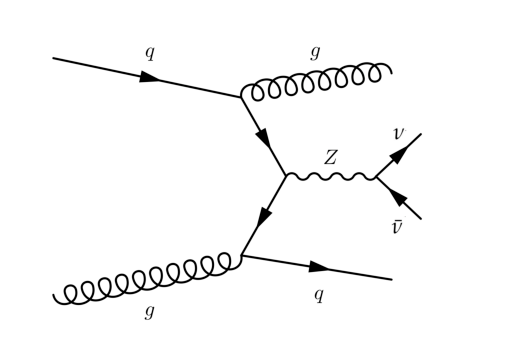
\includegraphics[width=0.45\textwidth]{QCDV2j_Feynman.pdf}
    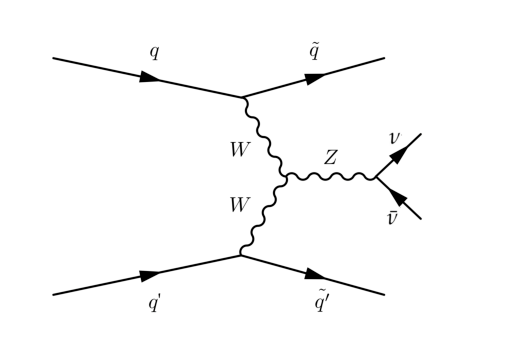
\includegraphics[width=0.45\textwidth]{VBFV2j_Feynman.pdf}
    \caption{Feynman diagrams showing the electroweak (left) and strong (right) production of a $\textrm{Z}$ boson, which decays into
    a pair of neutrinos. Two hadronic jets are also produced in the final state, making such processes an irreducible background
    in the VBF $\hinv$ analysis.}
    \label{fig:zvv_bkg_feynman}
\end{figure}

Another important background comes from the $\Wlvjets$ process, where a $\textrm{W}$ boson is produced and decays leptonically,
together with the presence of two hadronic jets in the final state.
This is not an irreducible background however, due to the fact that rejecting events with reconstructed leptons
will significantly suppress this process. Because of this, a lepton veto is imposed in the signal region, where  
events containing one or more loose muons or electrons with $\pt >10$ GeV, or hadronically decaying $\tau$ 
leptons with $\pt>20$ GeV are rejected\footnote{To be more precise, for events in MC simulation, 
instead of directly rejecting an event due to
a lepton in the final state, a veto weight $\omega$ is applied that depends on the kinematics of final state lepton(s), where
$\omega \approx 0$ in the presence of one or more reconstructed leptons. In observed data, no such reweighting is done and
the hard-lepton-veto is still applied. Please see Sec.~\ref{subsec:veto_weight_reweighting}
for details.}. 

Events that contain a loose, isolated photon with $\pt>15$ GeV and $|\eta| < 2.5$ are also rejected. 
This helps to suppress electroweak (EWK) backgrounds in which a photon is radiated from the initial state.
To reduce the contamination from top quark backgrounds, events are 
rejected\footnote{This requirement significantly suppresses the top quark backgrounds, due to its very large branching fraction
to final states with b quarks (\textit{i.e.,} $\textrm{BR}(\textrm{t} \rightarrow \textrm{W}^{+} \textrm{b}) \approx 96\%$).} 
if they contain a b-tagged jet with $\pt > 20$ GeV and $|\eta| < 2.4$. 
These jets are identified using the DeepCSV algorithm~\cite{CMS_NOTE_2018-323,Sirunyan:2017ezt}, 
adopting the ``medium'' working point, which corresponds to correctly identifying a jet originating from a bottom quark with 
a probability of 80\% and misidentifying a jet originating from a charm quark (light-flavor jet) with a probability of 12 (2)\%.

Last source of background is the QCD multijet events, with $\ptmiss$ arising from mismeasurements of the jet momenta. 
This background is suppressed by requiring the minimum
azimuthal angle between the \ptvecmiss direction and each of the first four leading jets with $\pt > 30$ GeV
and $|\eta| < 4.7$ to be larger than 0.5 radians. The QCD multijet background where one or more of the jet(s) is forward (\textit{i.e.,} $|\eta|>3$)
is further suppressed by the application of dedicated HF cleaning cuts, described in Sec.~\ref{subsec:hfnoise}.

The selection requirements for the signal region in this analysis are summarized in Table~\ref{tab:selection_mtr}.

\begin{table*}[htb]
    \caption{Summary of the signal region selection requirements. Leading and subleading jets refer to the highest and second-highest \pt jets in the event.}
    \begin{center}
        \renewcommand{\arraystretch}{1}
        \resizebox{\textwidth}{!} {
            \begin{tabular}{l c c}
                Variable                           & Selection                       & Target background \\
                \hline
                Muon (electron) veto               & $\pt > 10$ GeV, $|\eta| < 2.4 (2.5)$  & \Zlljets,~\Wlvjets \\
                $\tau$ lepton veto                 & $\pt > 20$ GeV, $|\eta| < 2.3$        & \Zlljets,~\Wlvjets  \\
                Photon veto                        & $\pt > 15$ GeV, $|\eta| < 2.5$        & \phojets \\
                Bottom jet veto                    & DeepCSV medium $< 0.4941 / 0.4184$ (2017 / 2018) &  Top quark \\
                                                    & for all jets with $\pt > 20$ GeV, $|\eta| < 2.4$ & \\
                $\ptmiss$                          & ${>} 250$ GeV                           & QCD, top quark, \Zlljets \\
                $\Delta\phi$($\ptvecjet$,$\ptvecmiss$)   &  $ {>} 0.5$ radians               & QCD \\
                Two leading jet IDs                 & POG tight ID, CHF$>0.1$, NHF$<0.8$ & Noise \\
                HF-noise rejection                  & Cuts on HF shape variables, $\sieie, \sipip$ and HF central strip size & HF noise \\
                $\Delta\ptmiss(\text{PF},\text{Calo})$ / recoil & $<0.5$ & Noise \\
                Leading AK4 jet $\pt$ and $\eta$     & ${>} 80$ GeV and $ |\eta| < 4.7$      & All \\
                Subleading AK4 jet $\pt$ and $\eta$   & ${>} 40$ GeV and $ |\eta| < 4.7$      & All \\
                $\mjj$                               & ${>} 200$ GeV  \\       
                $\detajj$                            & ${>} 1.0$  \\
                $\dphijj$                            & ${<} 1.5$  \\
            \end{tabular}
        }
        \label{tab:selection_mtr}
    \end{center}
\end{table*}

It should be noted that the selections listed in Table.~\ref{tab:selection_mtr} refer to one of the two event selection categories in the analysis,
the MET-triggered (MTR) category. In addition to the MTR category, there is another orthogonal event selection category called the 
VBF-triggered (VTR) category \cite{VBFHinvAnalysisPaper}.
Events in this category are collected using different HLT paths that require the presence of two energetic jets in the final state, and have 
$160 < \ptmiss < 250$ GeV, hence the orthogonality to the MTR category being considered here ($\ptmiss > 250$ GeV). 
For the purposes of this thesis, the VTR category won't be discussed in detail, but the combined
results with the VTR category will be mentioned in Sec.~\ref{chapter:results}. 

Figs.~\ref{fig:SR_pre_vbfhinv_2017_mtr},~\ref{fig:SR_jets_vbfhinv_2017_mtr}, and~\ref{fig:SR_eta_vbfhinv_2017_mtr} 
show the distribution of the $\ptmiss$, $\mjj$, $\detajj$ and $\dphijj$ of the VBF jet pair (two highest-$\pt$ jets), the $\pt$ and $\eta$ distributions 
of the leading and subleading jets, and the $\eta$ distributions of the most central and most forward jets, respectively, for events
passing the VBF signal region selection.
The same distributions are shown for the 2018 samples in Figs.~\ref{fig:SR_pre_vbfhinv_2018_mtr},~\ref{fig:SR_jets_vbfhinv_2018_mtr},
and~\ref{fig:SR_eta_vbfhinv_2018_mtr}.

\begin{figure}[htbp]
    \begin{center}
        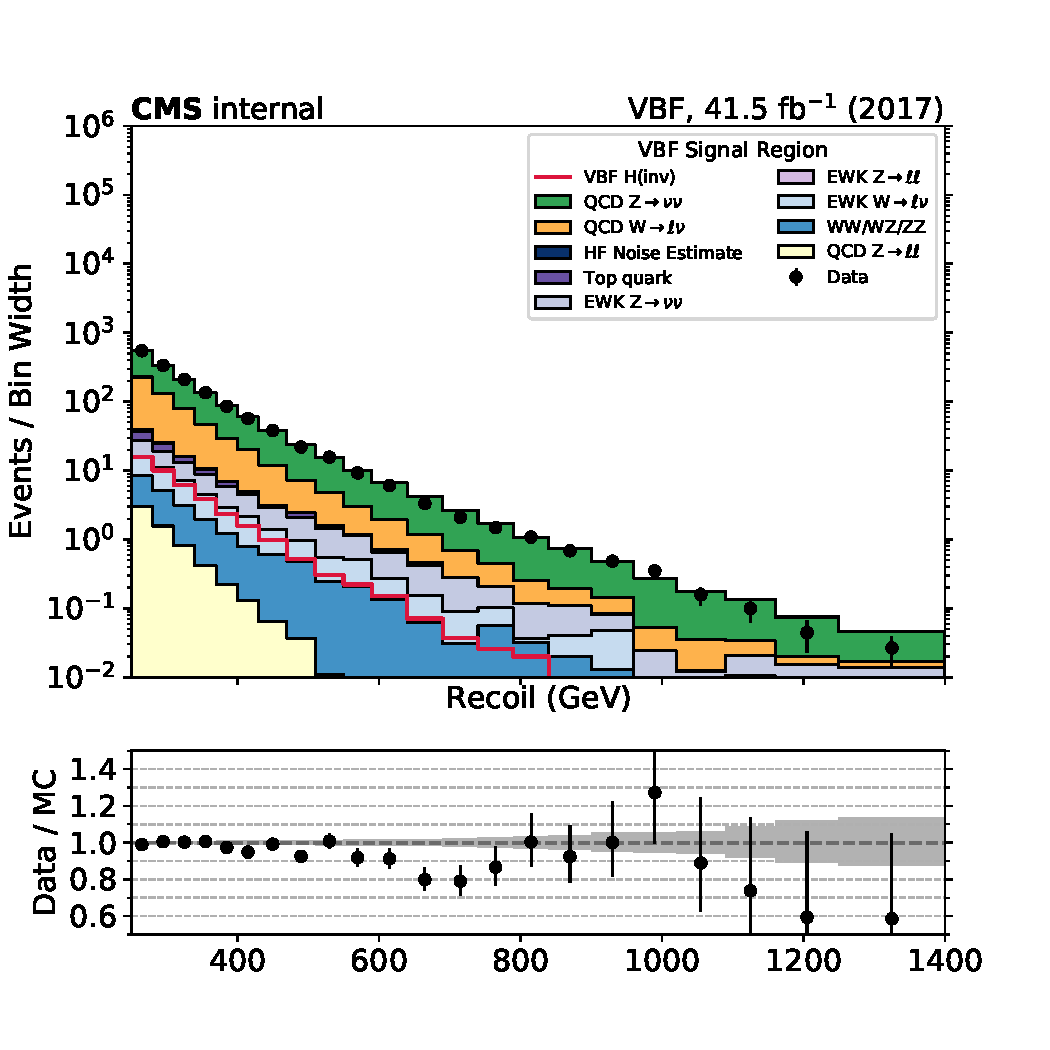
\includegraphics[width=0.49\textwidth]{\plotDir/sr_vbf/sr_vbf_data_mc_recoil_2017.pdf}
        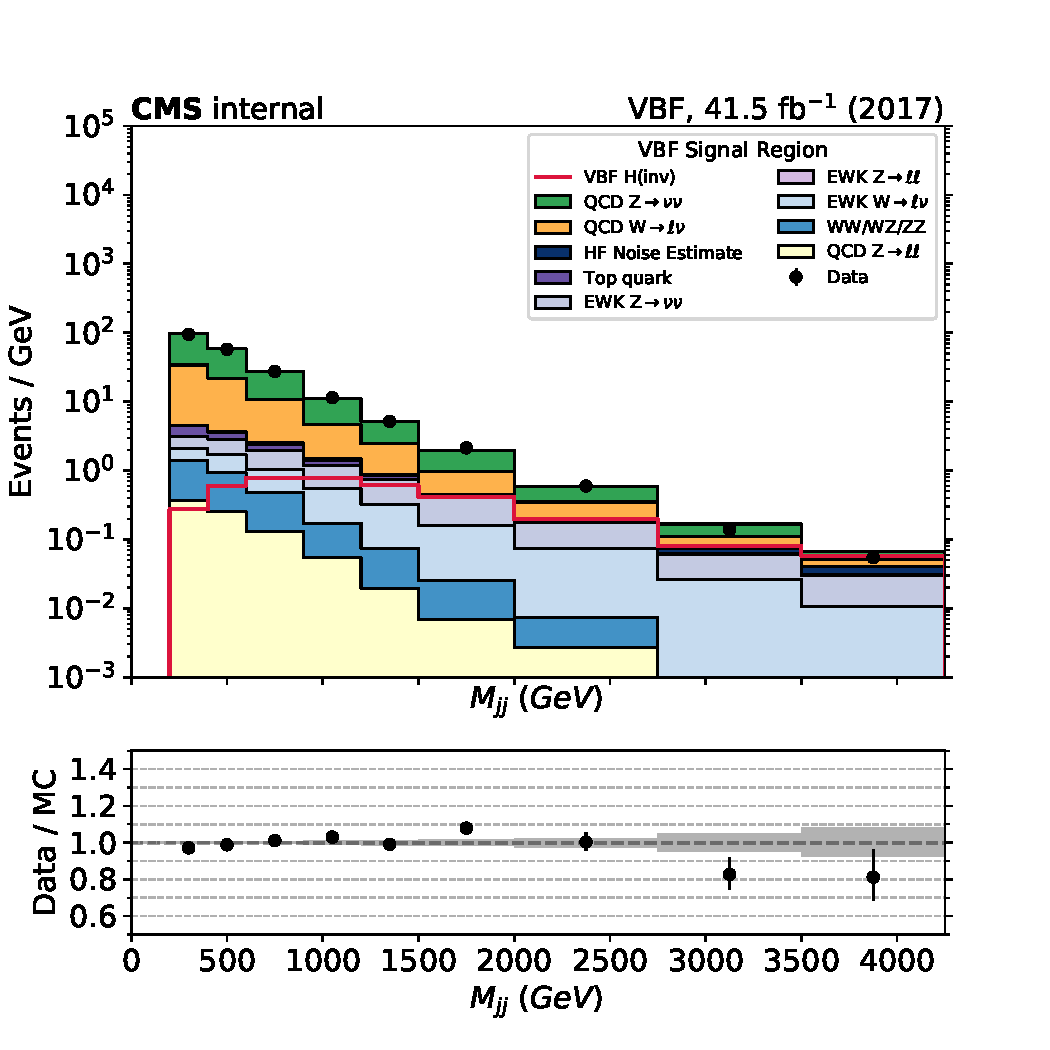
\includegraphics[width=0.49\textwidth]{\plotDir/sr_vbf/sr_vbf_data_mc_mjj_2017.pdf} \\
        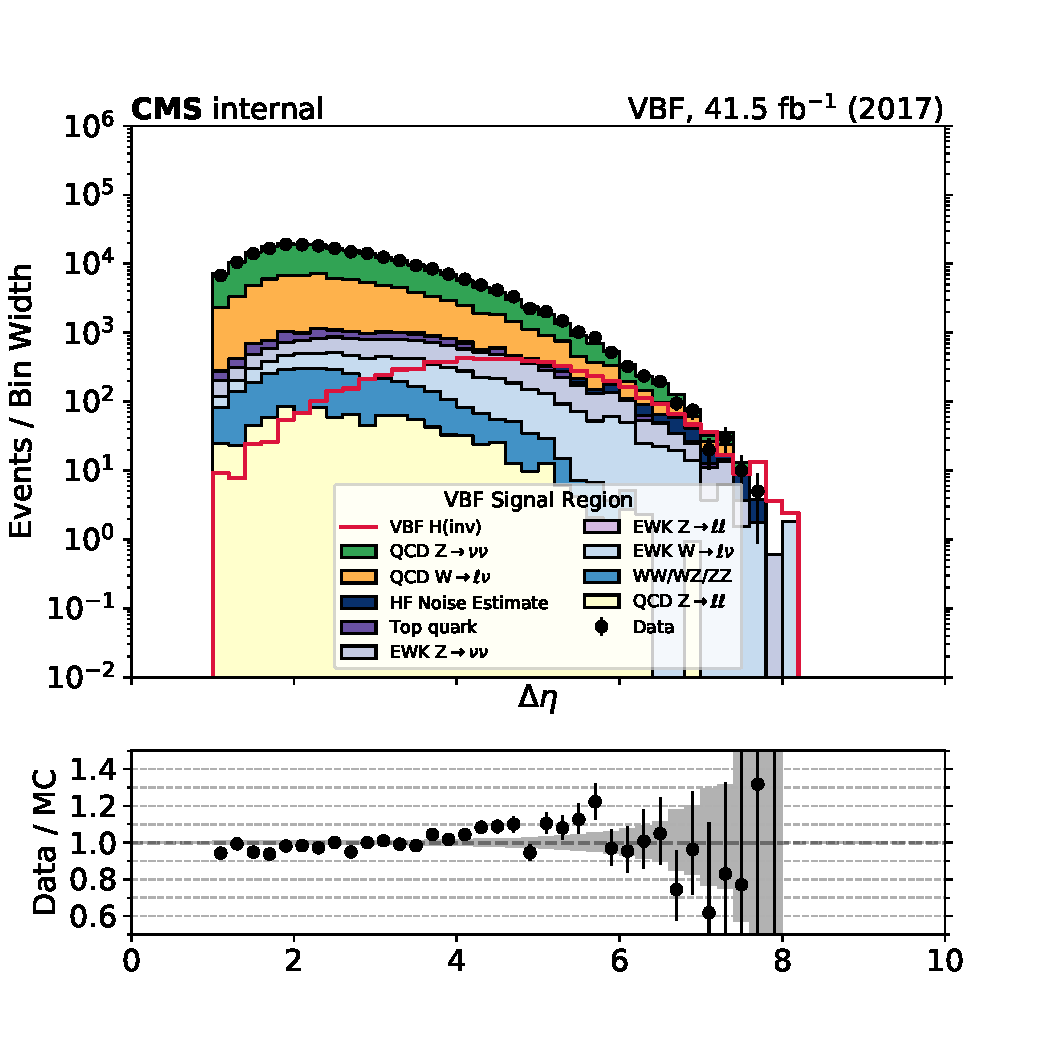
\includegraphics[width=0.49\textwidth]{\plotDir/sr_vbf/sr_vbf_data_mc_detajj_2017.pdf}
        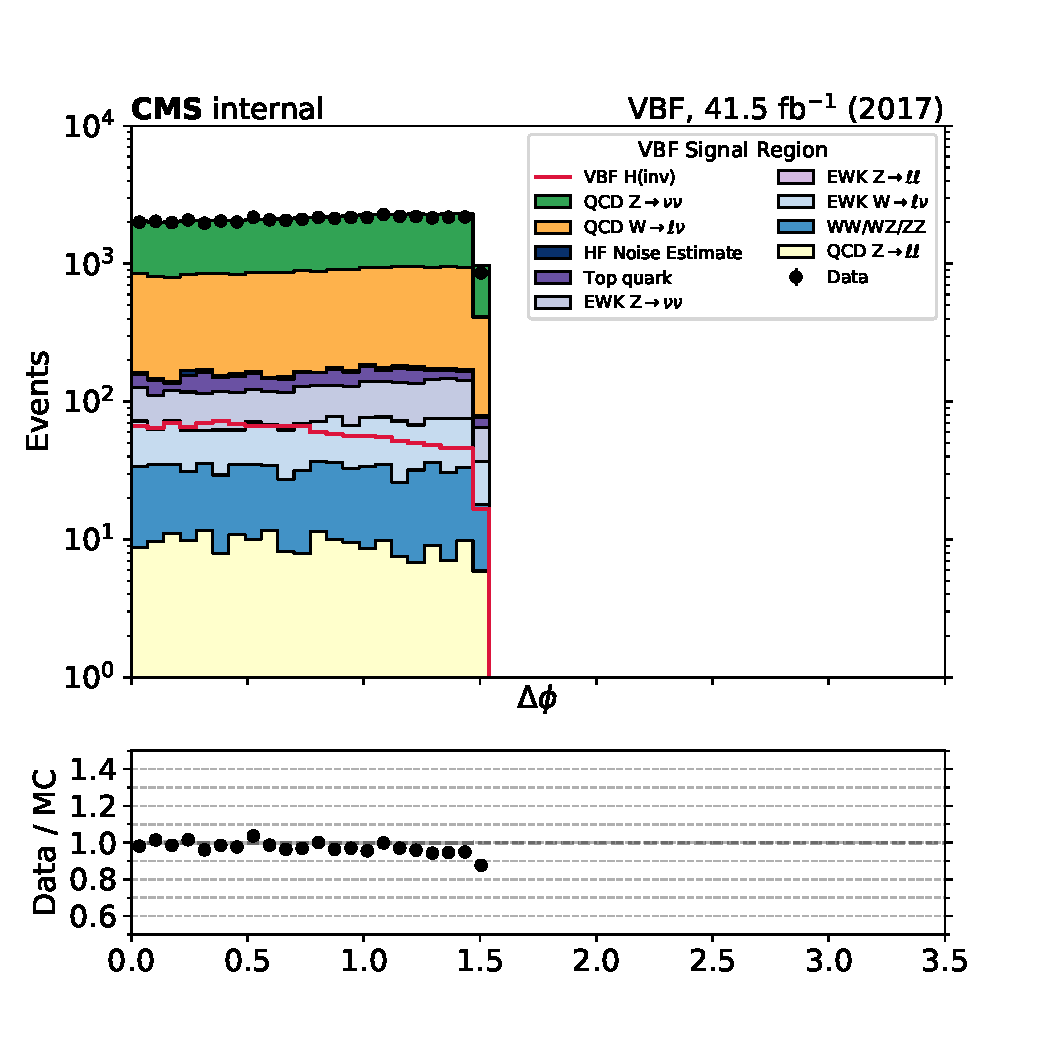
\includegraphics[width=0.49\textwidth]{\plotDir/sr_vbf/sr_vbf_data_mc_dphijj_2017.pdf}
        
    \end{center}
    \caption{Recoil distribution, $\mjj$ distribution, $\detajj$ and $\dphijj$
    distribution in the VBF signal region, using 2017 dataset.}
    \label{fig:SR_pre_vbfhinv_2017_mtr}
\end{figure}

\begin{figure}[htbp]
    \begin{center}
        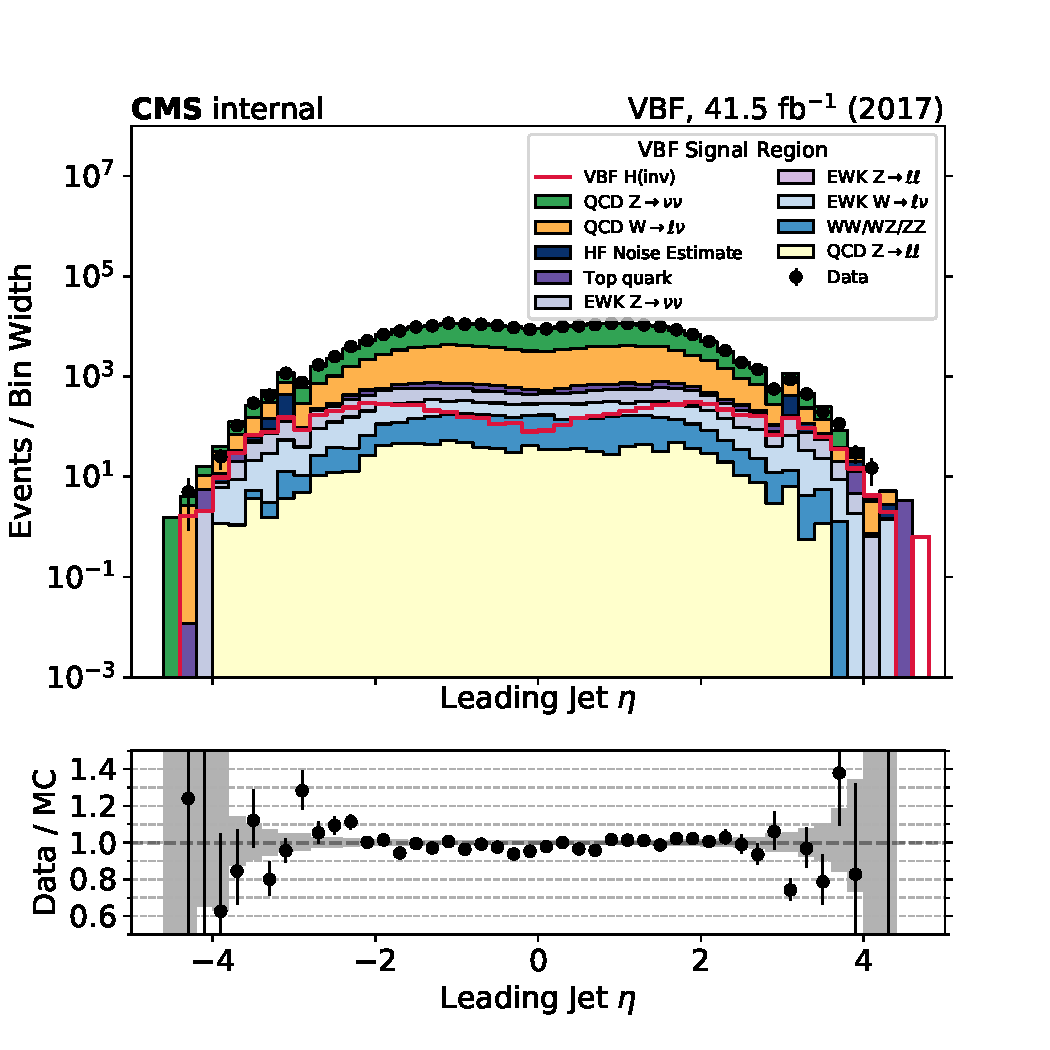
\includegraphics[width=0.49\textwidth]{\plotDir/sr_vbf/sr_vbf_data_mc_ak4_eta0_2017.pdf}
        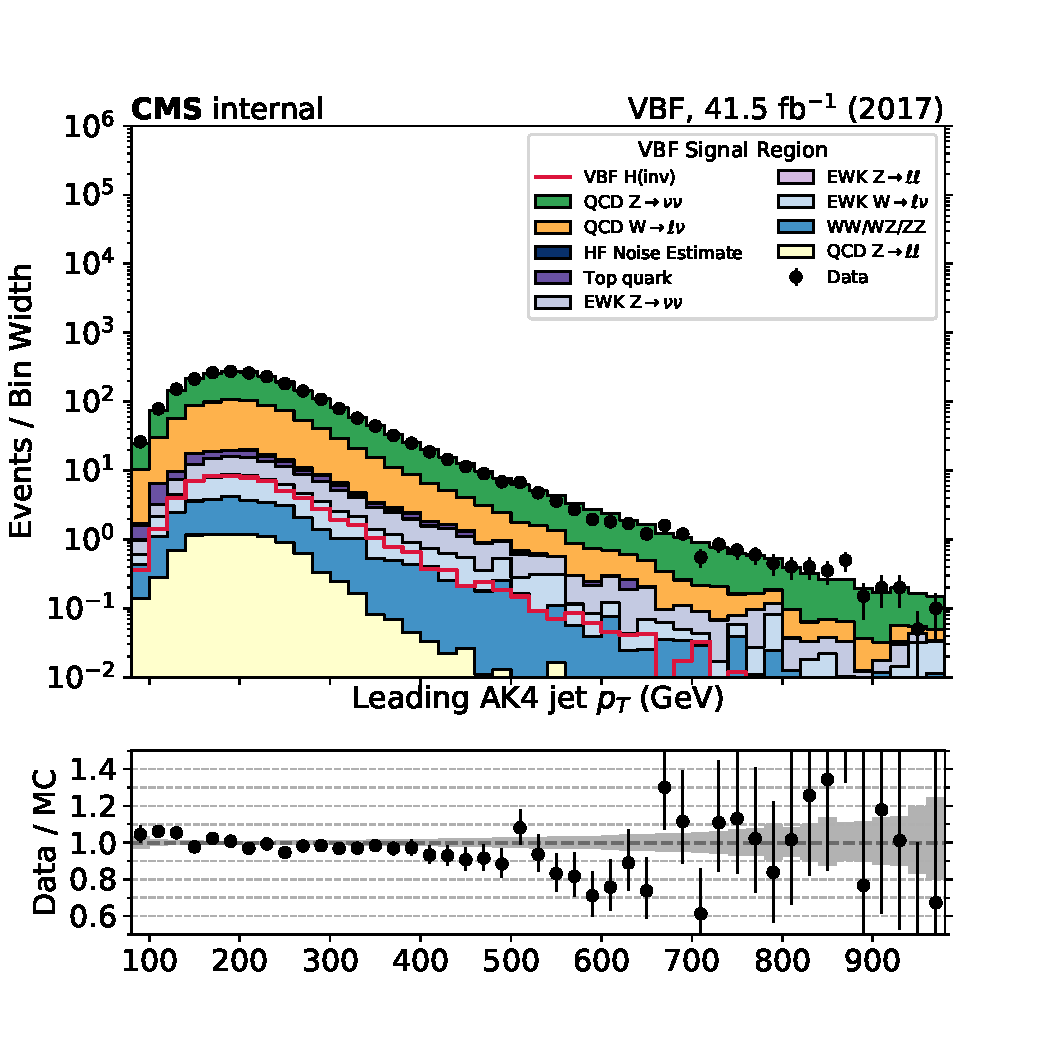
\includegraphics[width=0.49\textwidth]{\plotDir/sr_vbf/sr_vbf_data_mc_ak4_pt0_2017.pdf} \\
        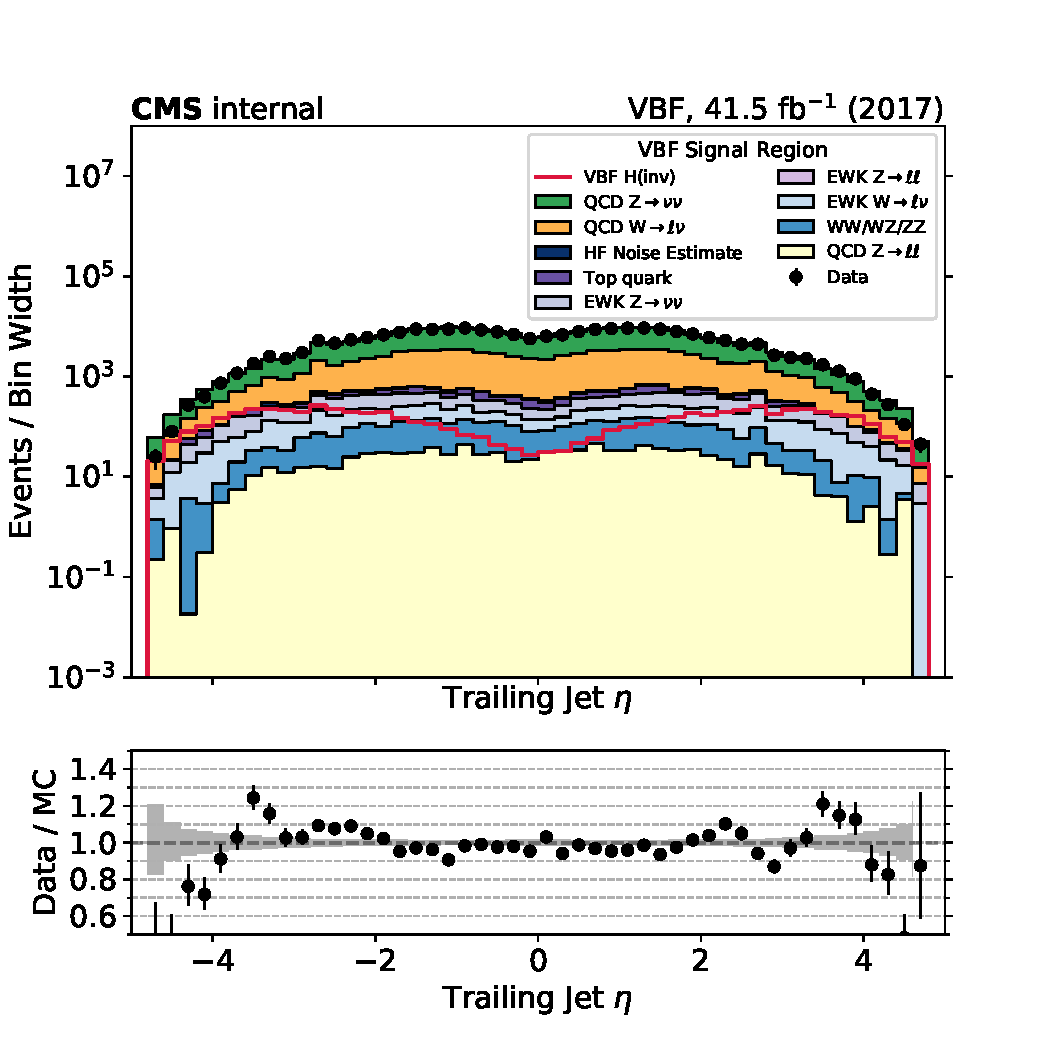
\includegraphics[width=0.49\textwidth]{\plotDir/sr_vbf/sr_vbf_data_mc_ak4_eta1_2017.pdf}
        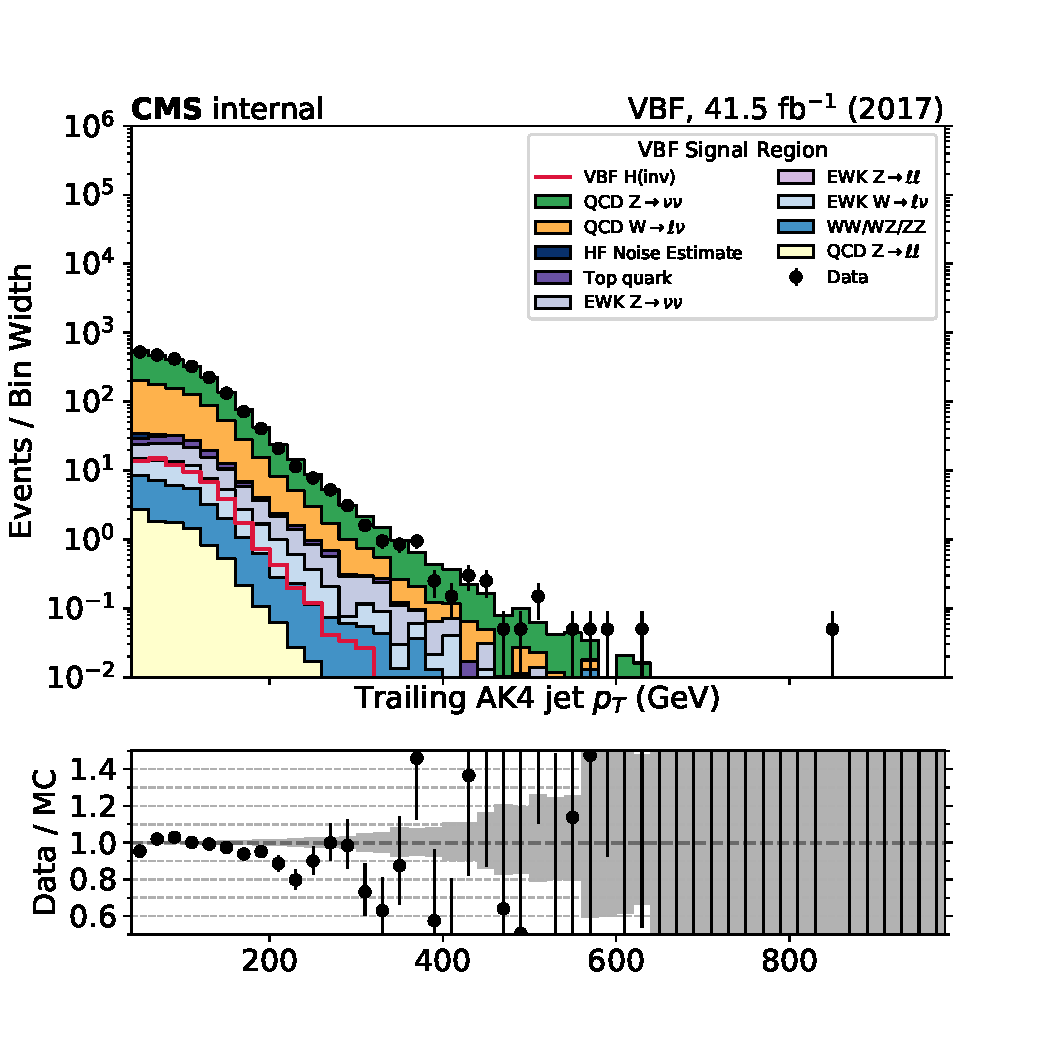
\includegraphics[width=0.49\textwidth]{\plotDir/sr_vbf/sr_vbf_data_mc_ak4_pt1_2017.pdf}
    \end{center}
    \caption{Leading and subleading jets $\pt$ and $\eta$ in the VBF signal region, using 2017 dataset.}
    \label{fig:SR_jets_vbfhinv_2017_mtr}
\end{figure}

\begin{figure}[htbp]
    \begin{center}
        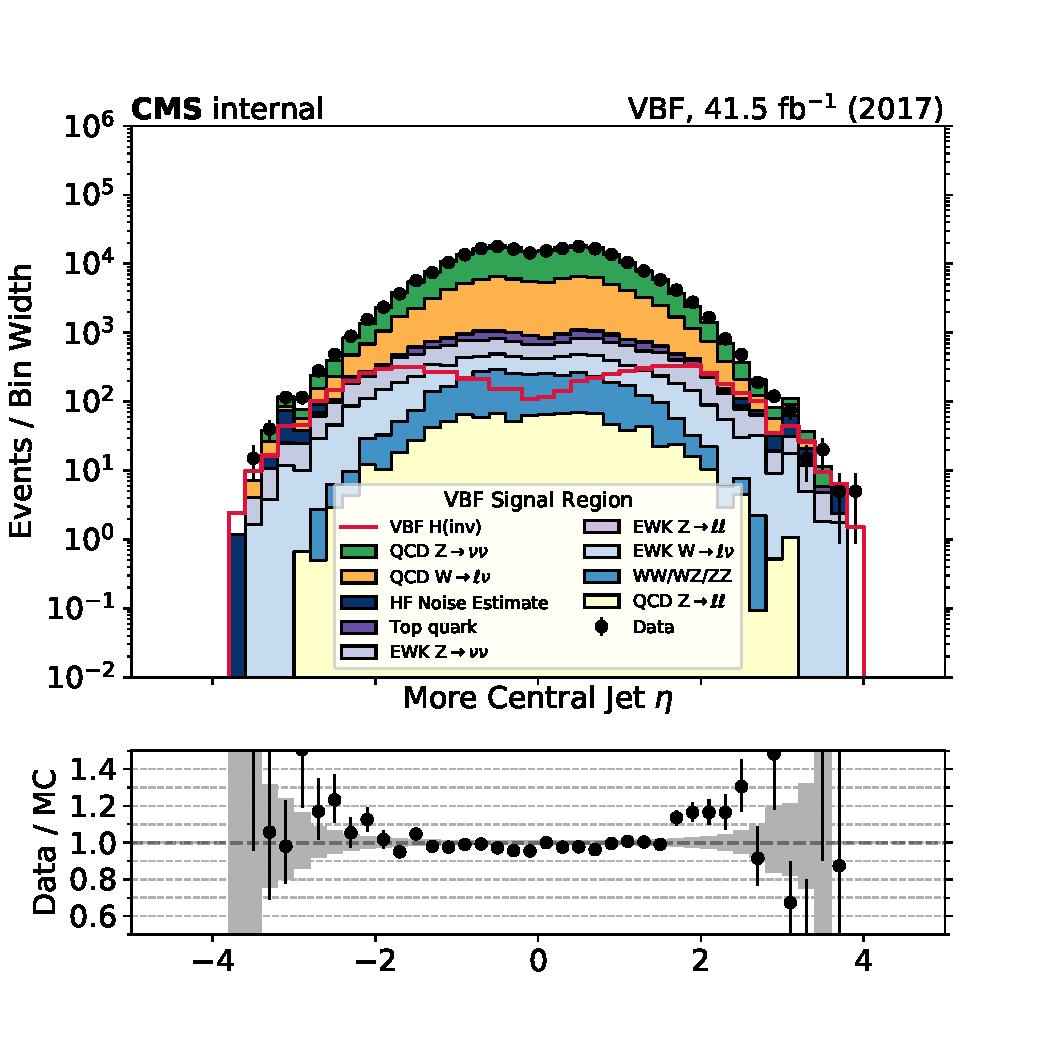
\includegraphics[width=0.49\textwidth]{\plotDir/sr_vbf/sr_vbf_data_mc_ak4_central_eta_2017.pdf}
        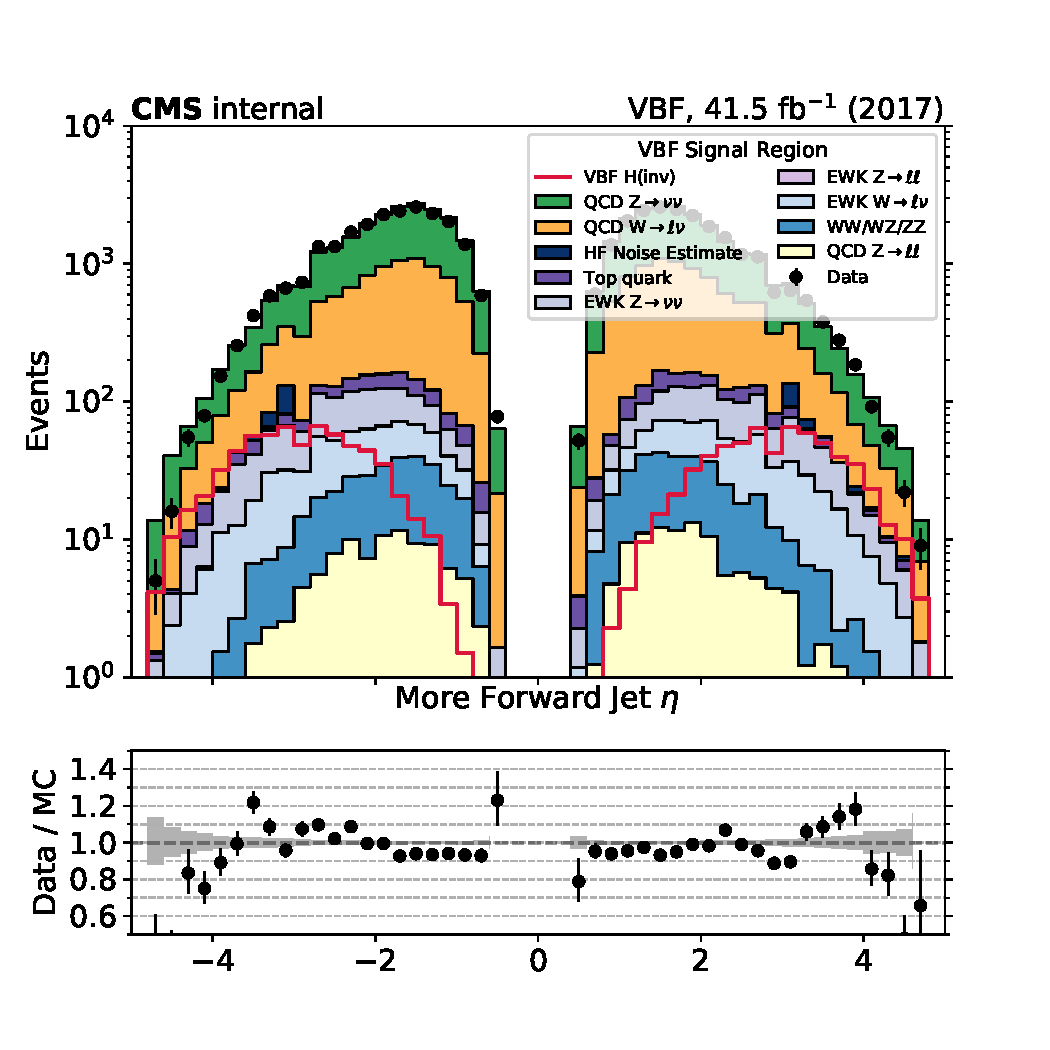
\includegraphics[width=0.49\textwidth]{\plotDir/sr_vbf/sr_vbf_data_mc_ak4_forward_eta_2017.pdf}
    \end{center}
    \caption{Most central (left) and most forward jets (right) $\eta$ of the VBF pair in the VBF signal region, using 2017 dataset.}
    \label{fig:SR_eta_vbfhinv_2017_mtr}
\end{figure}


% \begin{figure}[htbp]
%     \begin{center}
%         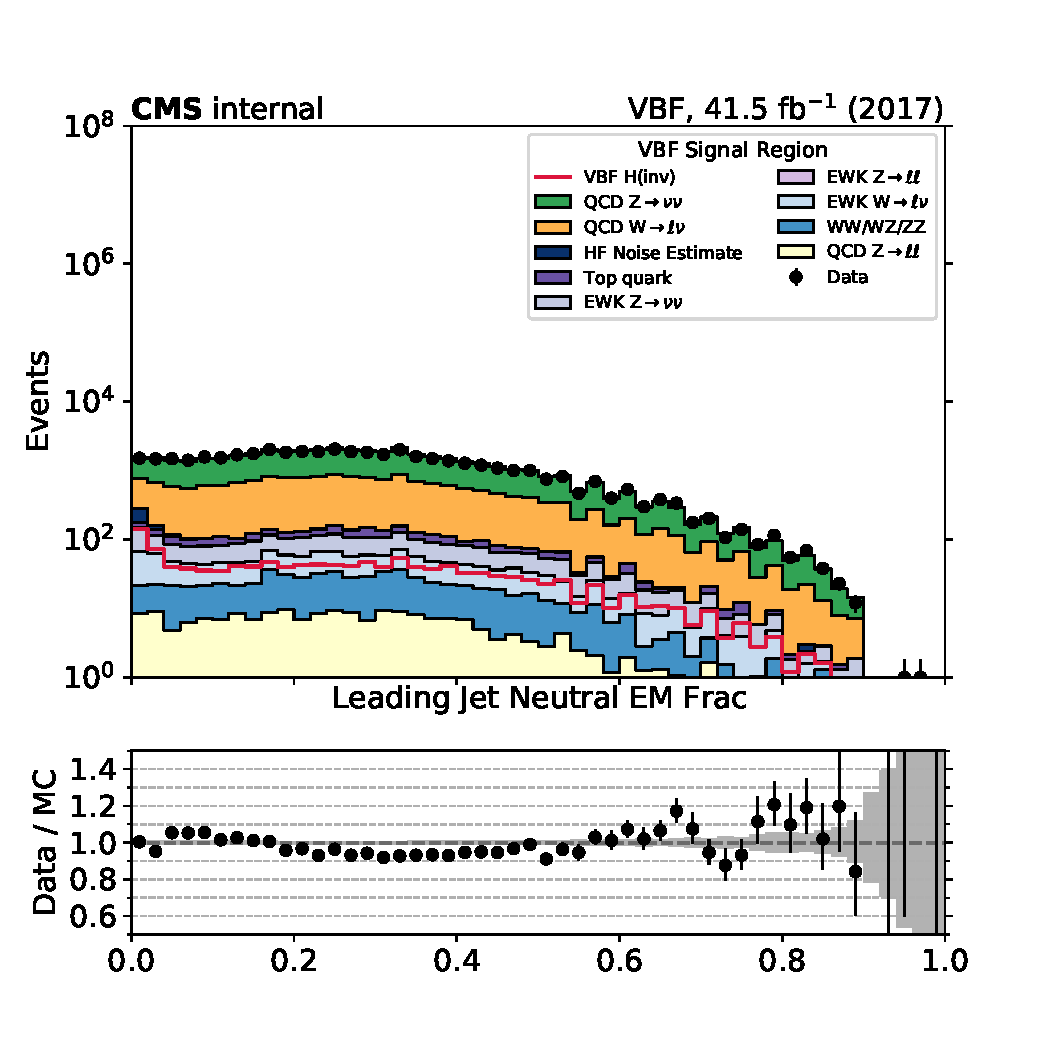
\includegraphics[width=0.49\textwidth]{\plotDir/sr_vbf/sr_vbf_data_mc_ak4_nef0_2017.pdf}
%         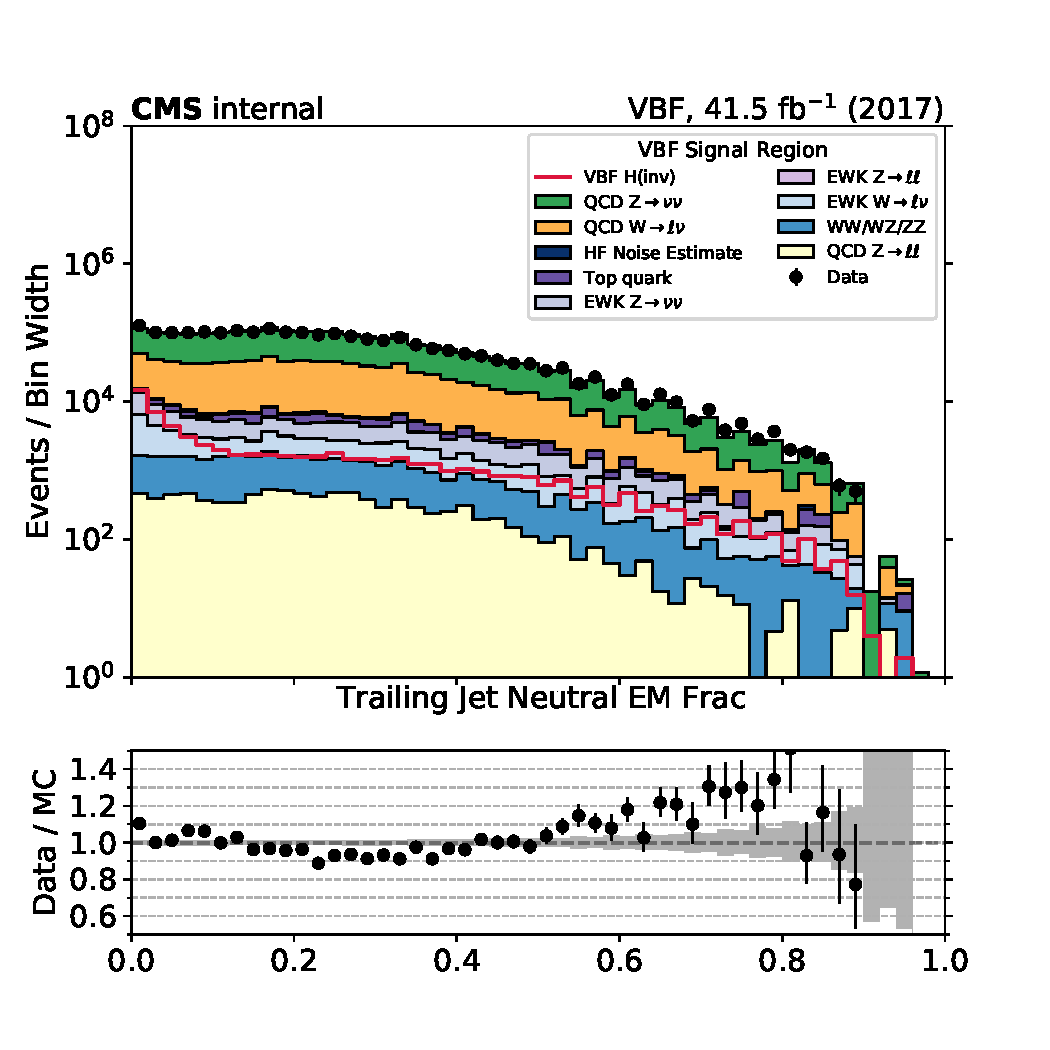
\includegraphics[width=0.49\textwidth]{\plotDir/sr_vbf/sr_vbf_data_mc_ak4_nef1_2017.pdf} \\
%         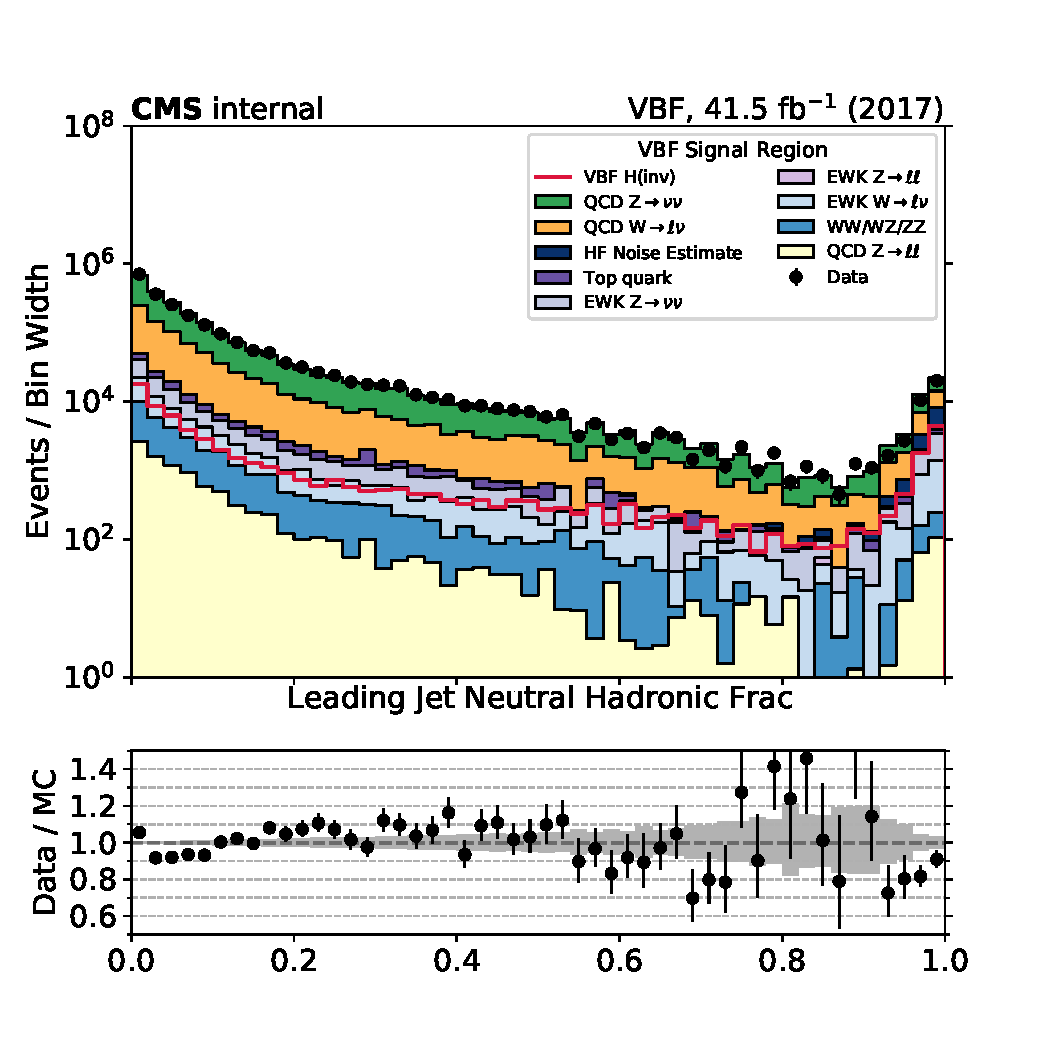
\includegraphics[width=0.49\textwidth]{\plotDir/sr_vbf/sr_vbf_data_mc_ak4_nhf0_2017.pdf}
%         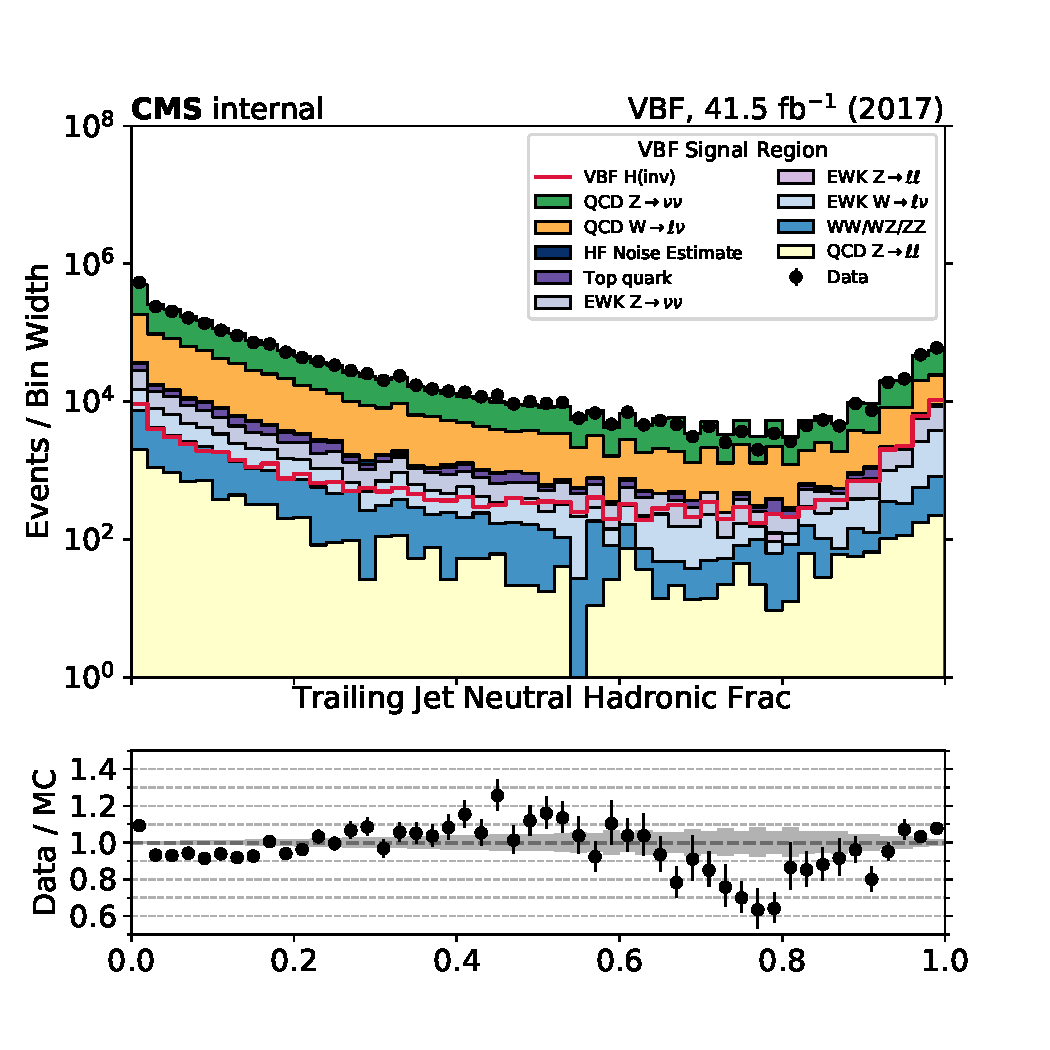
\includegraphics[width=0.49\textwidth]{\plotDir/sr_vbf/sr_vbf_data_mc_ak4_nhf1_2017.pdf} \\
%     \end{center}
%     \caption{Neutral electromagnetic energy fractions (top) and neutral hadron energy fractions for the leading two jets in the VBF signal region,
%     using 2017 dataset.}
%     \label{fig:SR_nhf_nef_2017_mtr}
% \end{figure}

% \begin{figure}[htbp]
%     \begin{center}
%         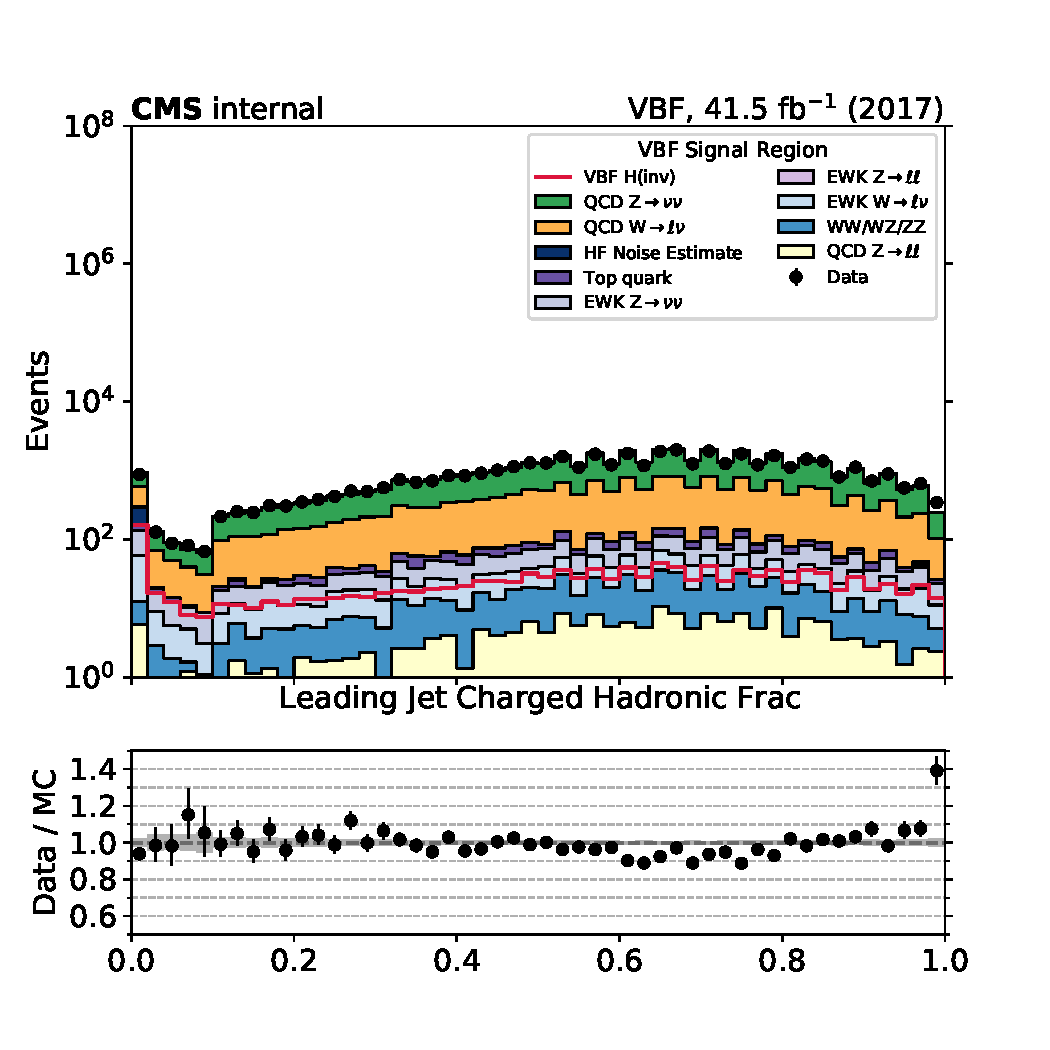
\includegraphics[width=0.49\textwidth]{\plotDir/sr_vbf/sr_vbf_data_mc_ak4_chf0_2017.pdf}
%         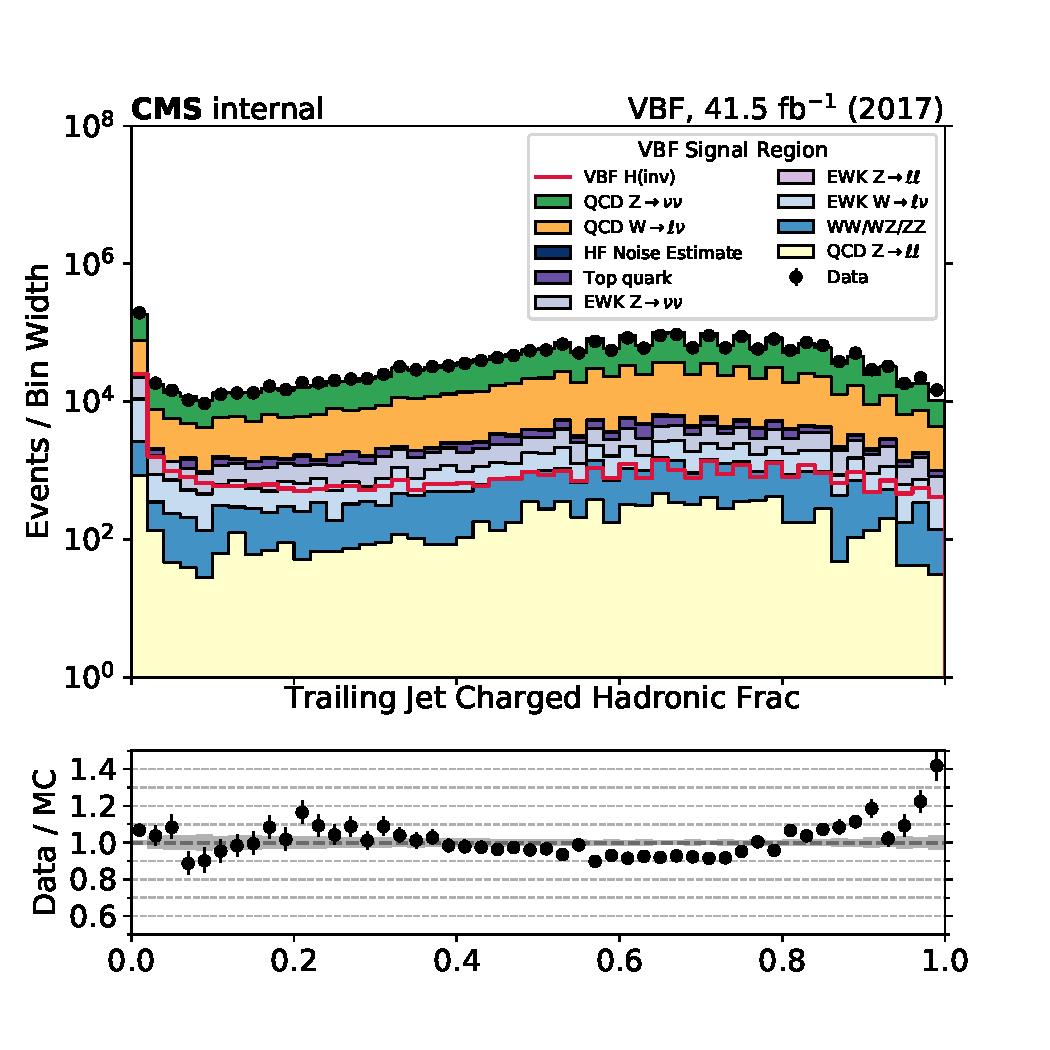
\includegraphics[width=0.49\textwidth]{\plotDir/sr_vbf/sr_vbf_data_mc_ak4_chf1_2017.pdf}
%     \end{center}
%     \caption{Charged hadronic energy fractions for the leading two jets in the VBF signal region,
%     using 2017 dataset.}
%     \label{fig:SR_chf_2017_mtr}
% \end{figure}

\begin{figure}[htbp]
    \begin{center}
        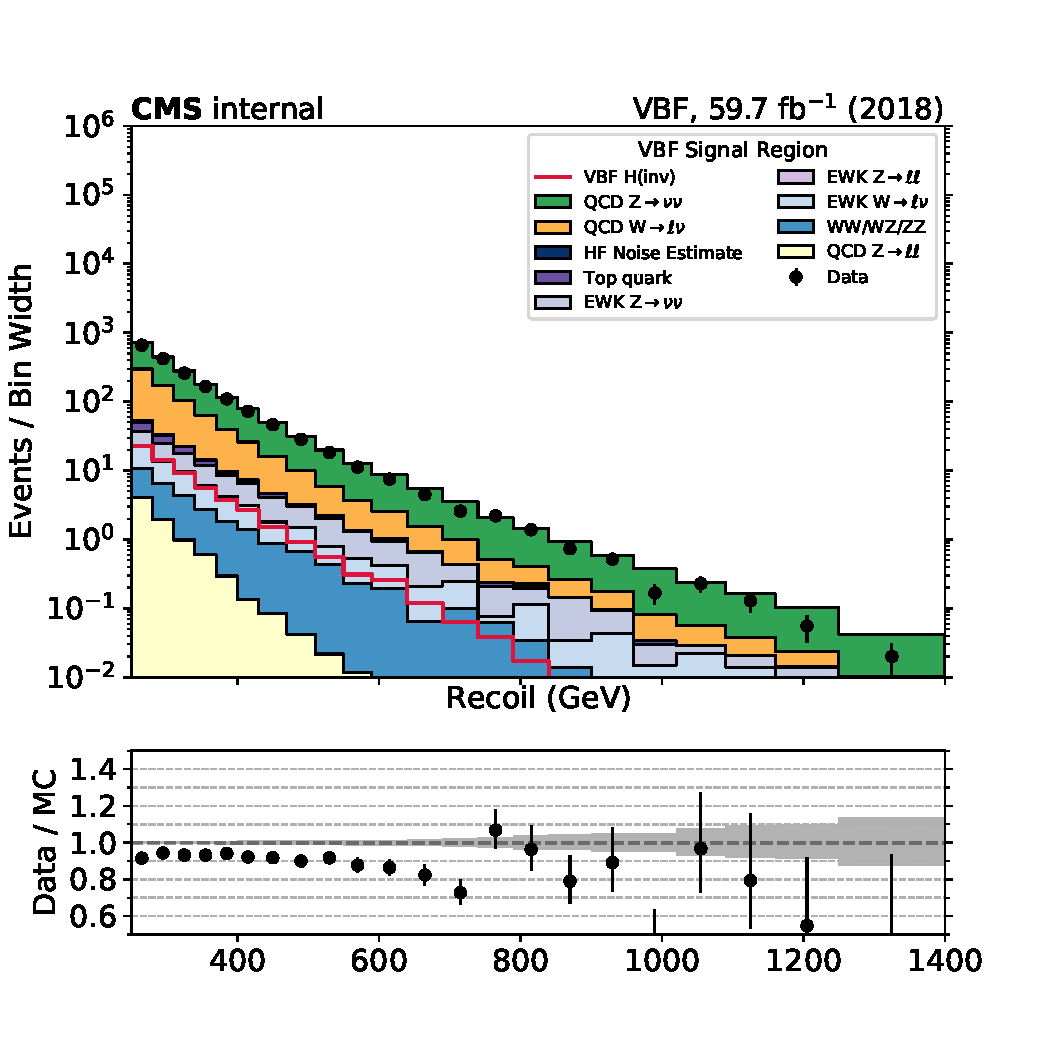
\includegraphics[width=0.49\textwidth]{\plotDir/sr_vbf/sr_vbf_data_mc_recoil_2018.pdf}
        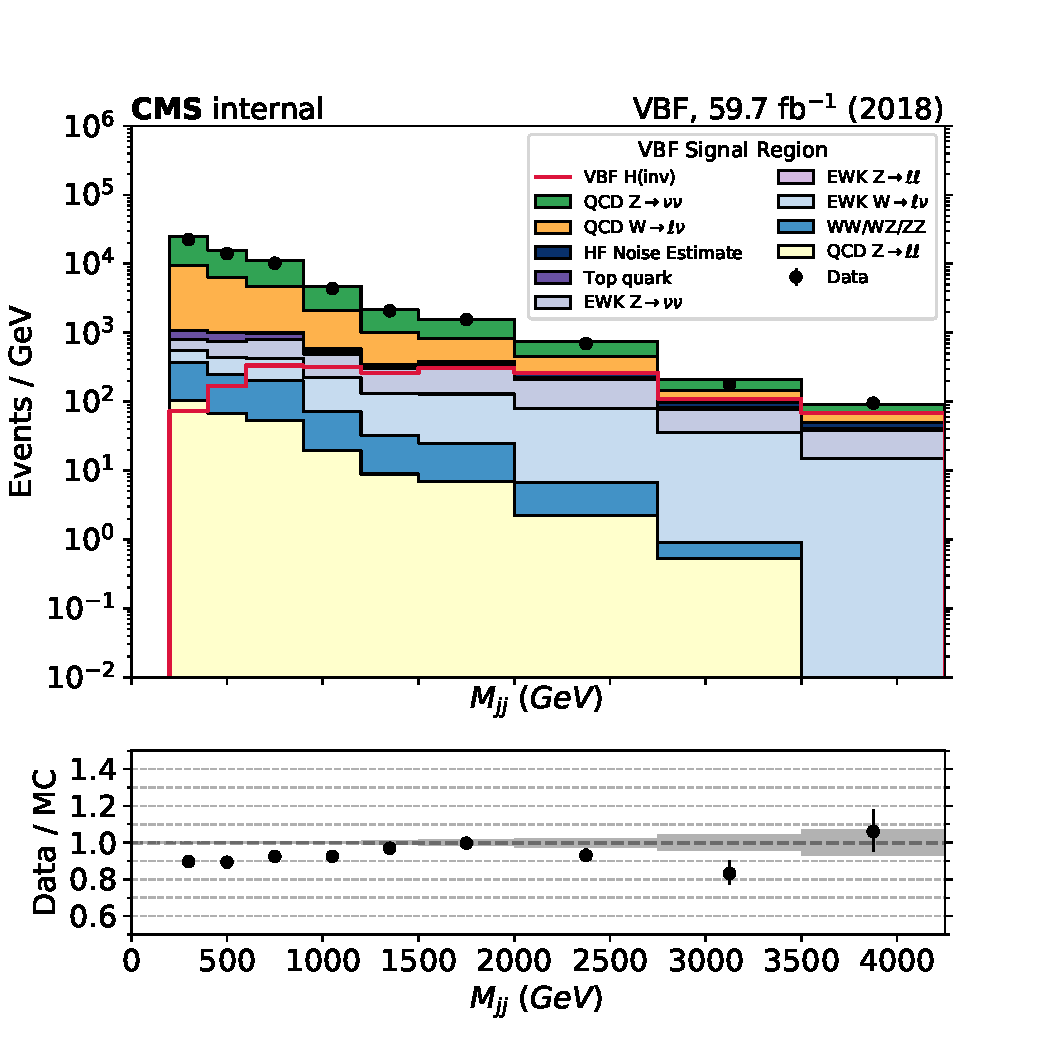
\includegraphics[width=0.49\textwidth]{\plotDir/sr_vbf/sr_vbf_data_mc_mjj_2018.pdf} \\
        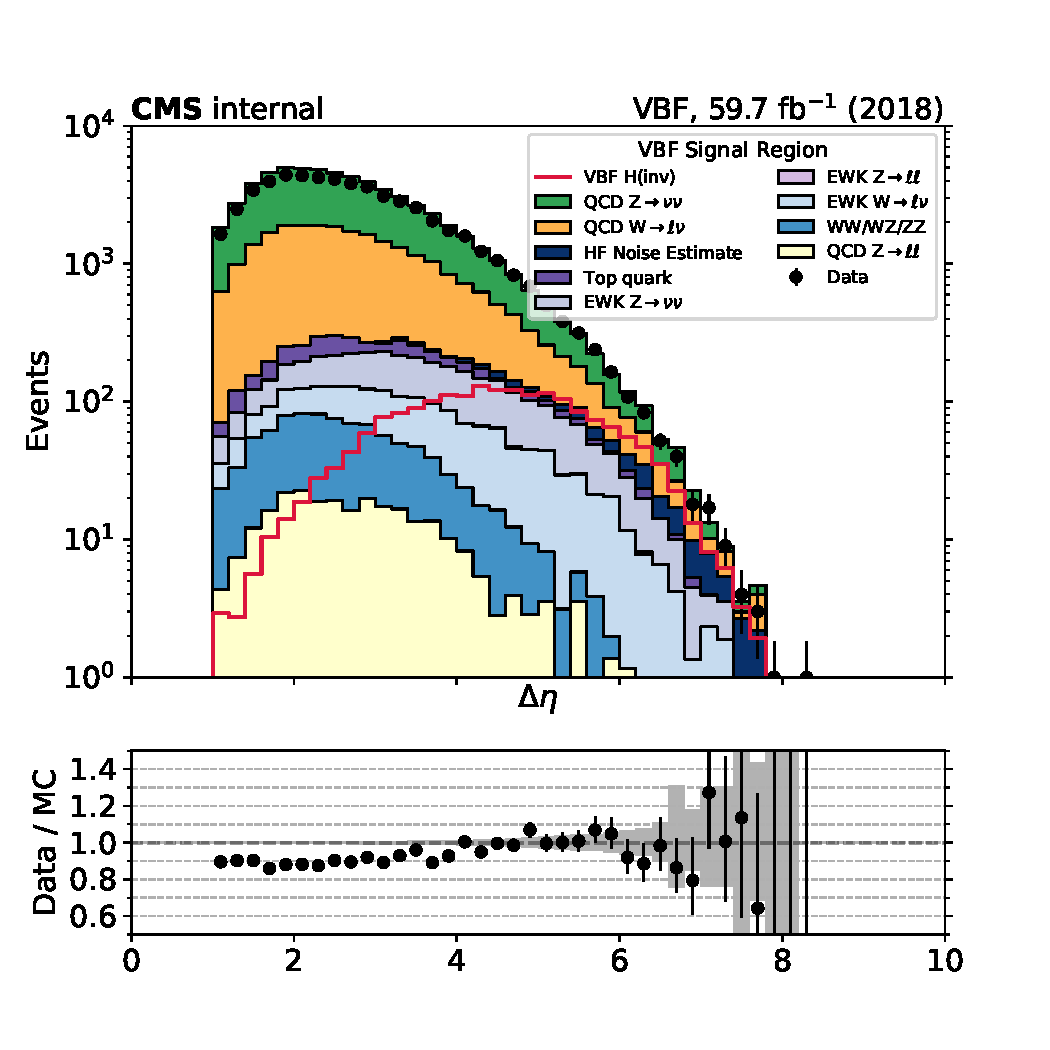
\includegraphics[width=0.49\textwidth]{\plotDir/sr_vbf/sr_vbf_data_mc_detajj_2018.pdf}
        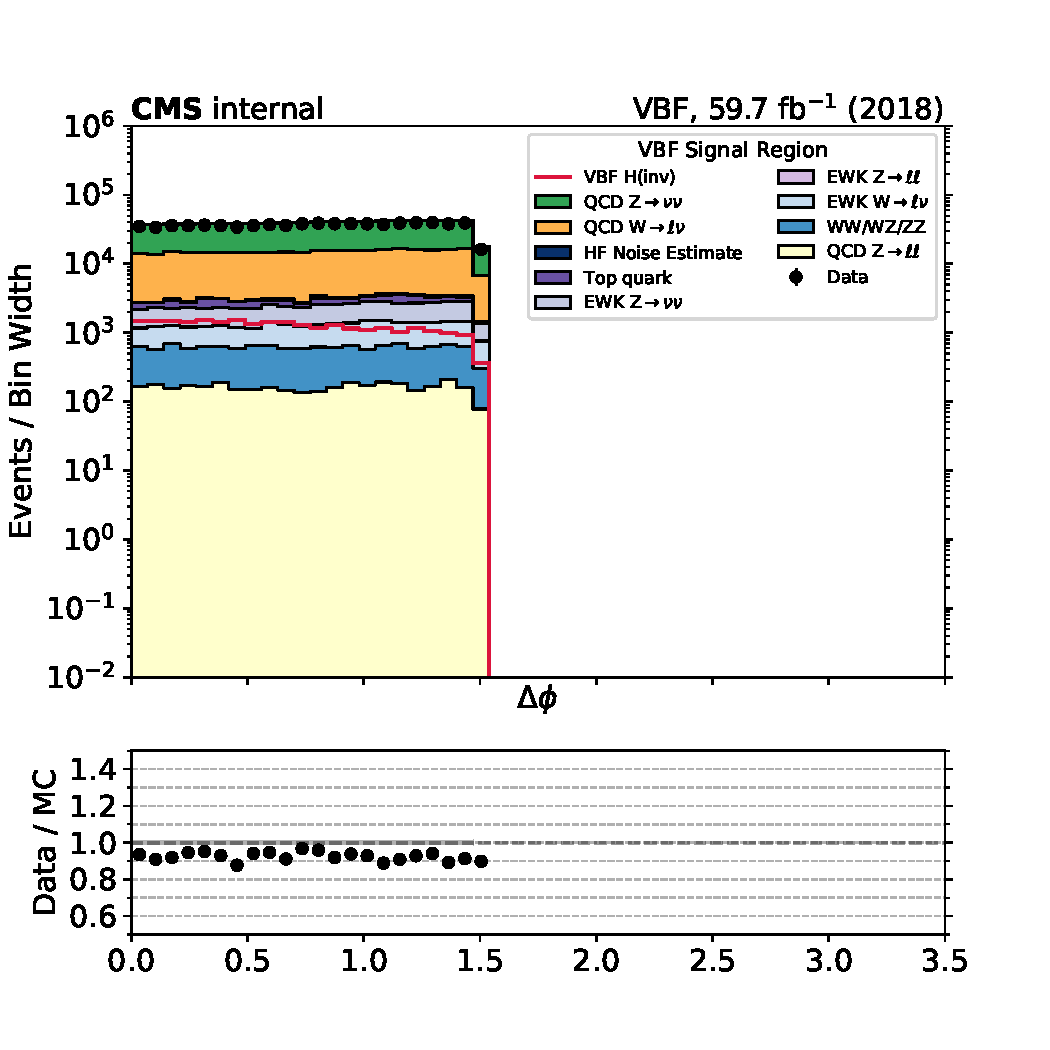
\includegraphics[width=0.49\textwidth]{\plotDir/sr_vbf/sr_vbf_data_mc_dphijj_2018.pdf}
    \end{center}
    \caption{Recoil distribution, $\mjj$ distribution, $\detajj$ and $\dphijj$
    distribution in the VBF signal region, using 2018 dataset.}
    \label{fig:SR_pre_vbfhinv_2018_mtr}
\end{figure}

\begin{figure}[htbp]
    \begin{center}
        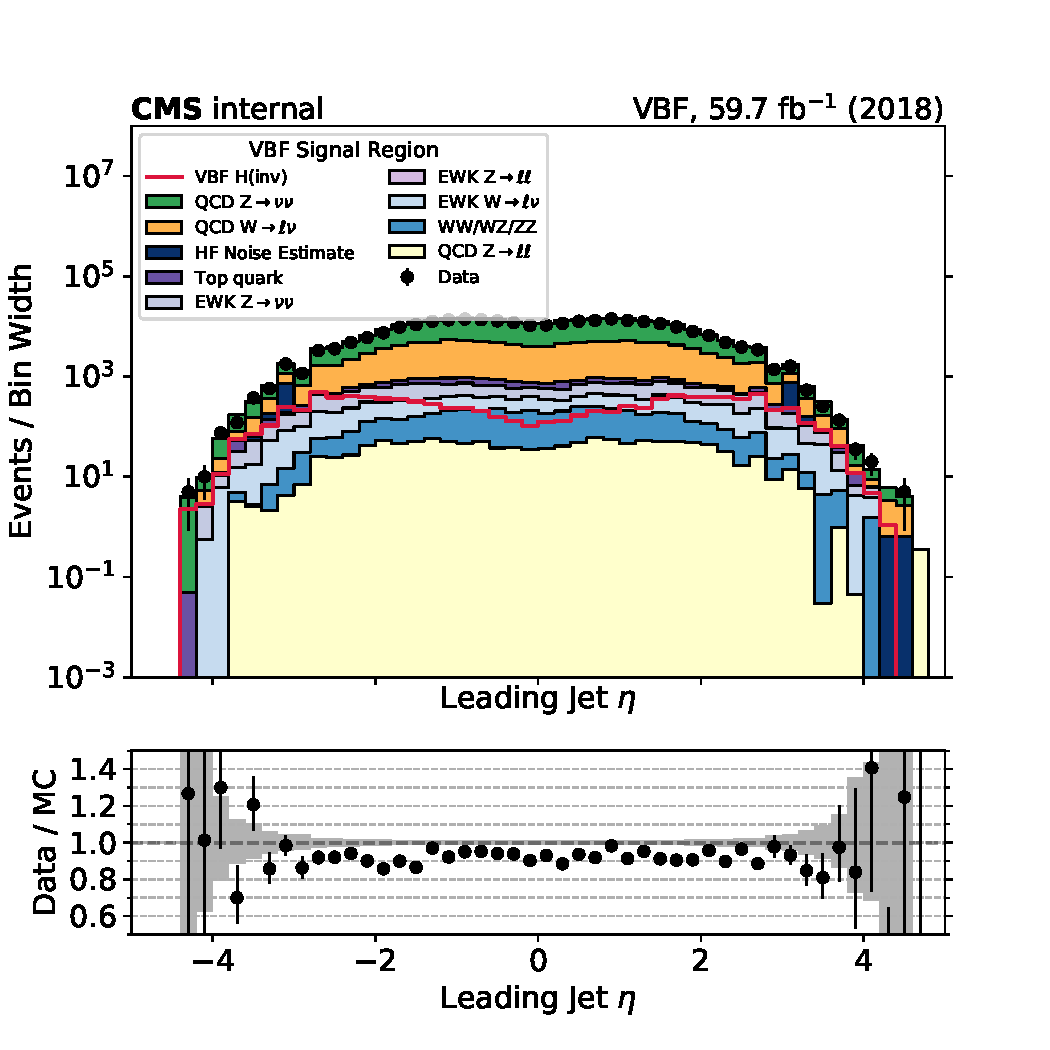
\includegraphics[width=0.49\textwidth]{\plotDir/sr_vbf/sr_vbf_data_mc_ak4_eta0_2018.pdf}
        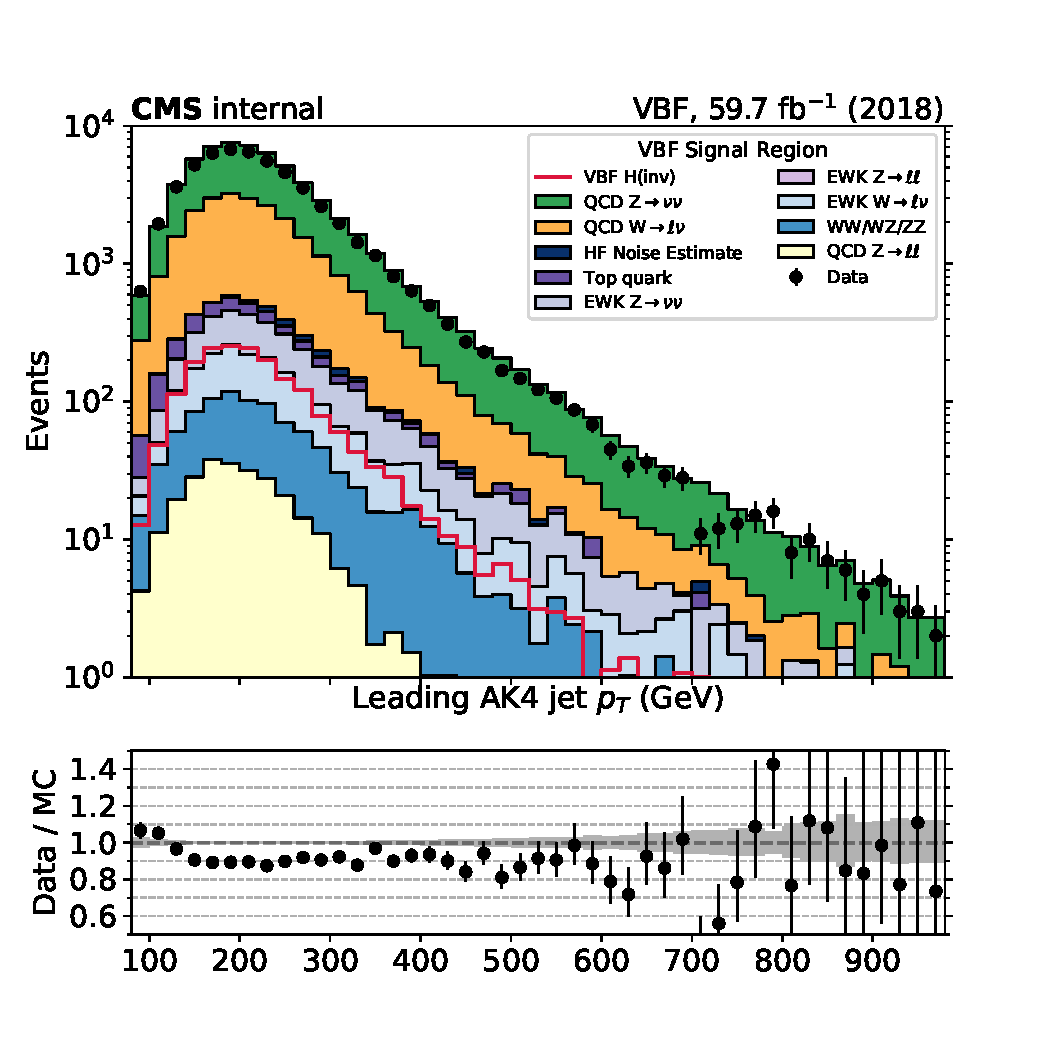
\includegraphics[width=0.49\textwidth]{\plotDir/sr_vbf/sr_vbf_data_mc_ak4_pt0_2018.pdf} \\
        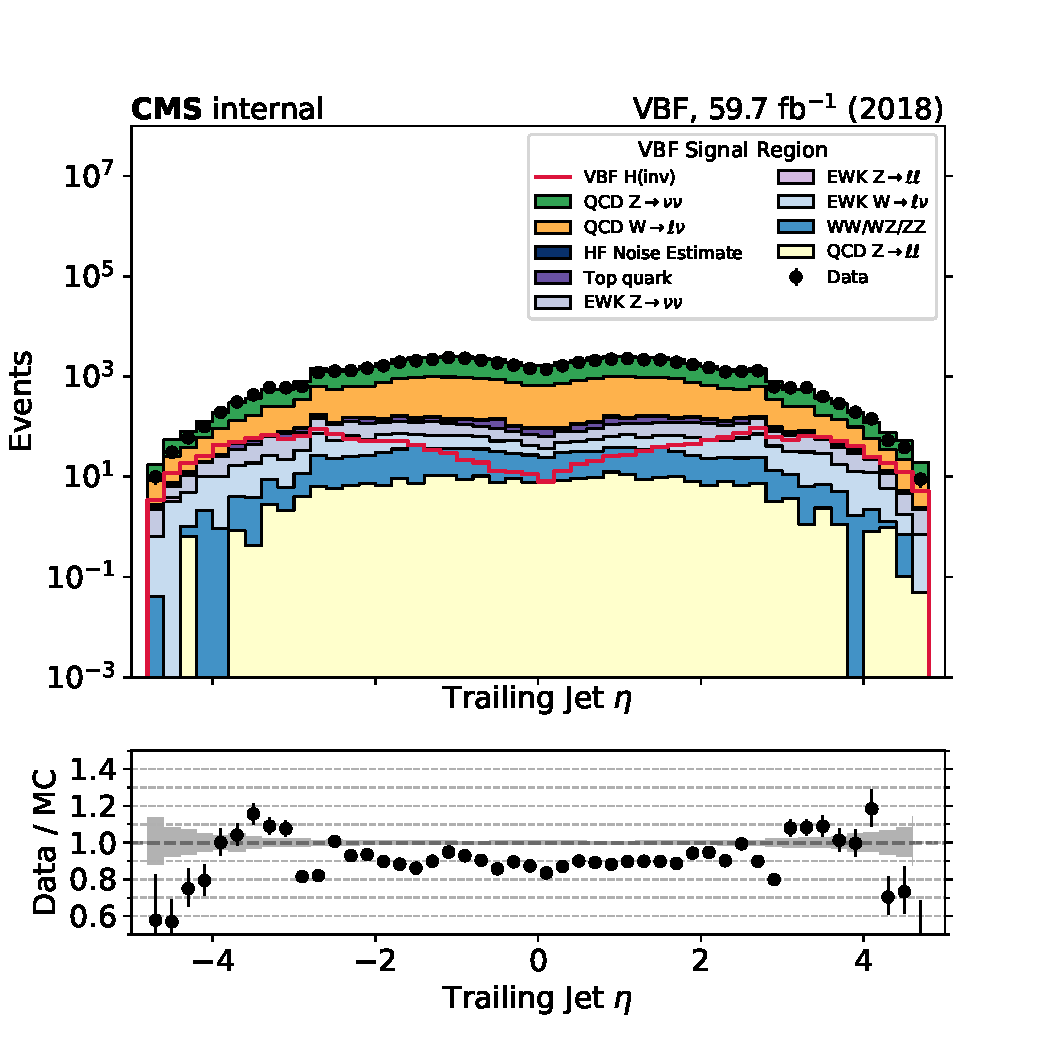
\includegraphics[width=0.49\textwidth]{\plotDir/sr_vbf/sr_vbf_data_mc_ak4_eta1_2018.pdf}
        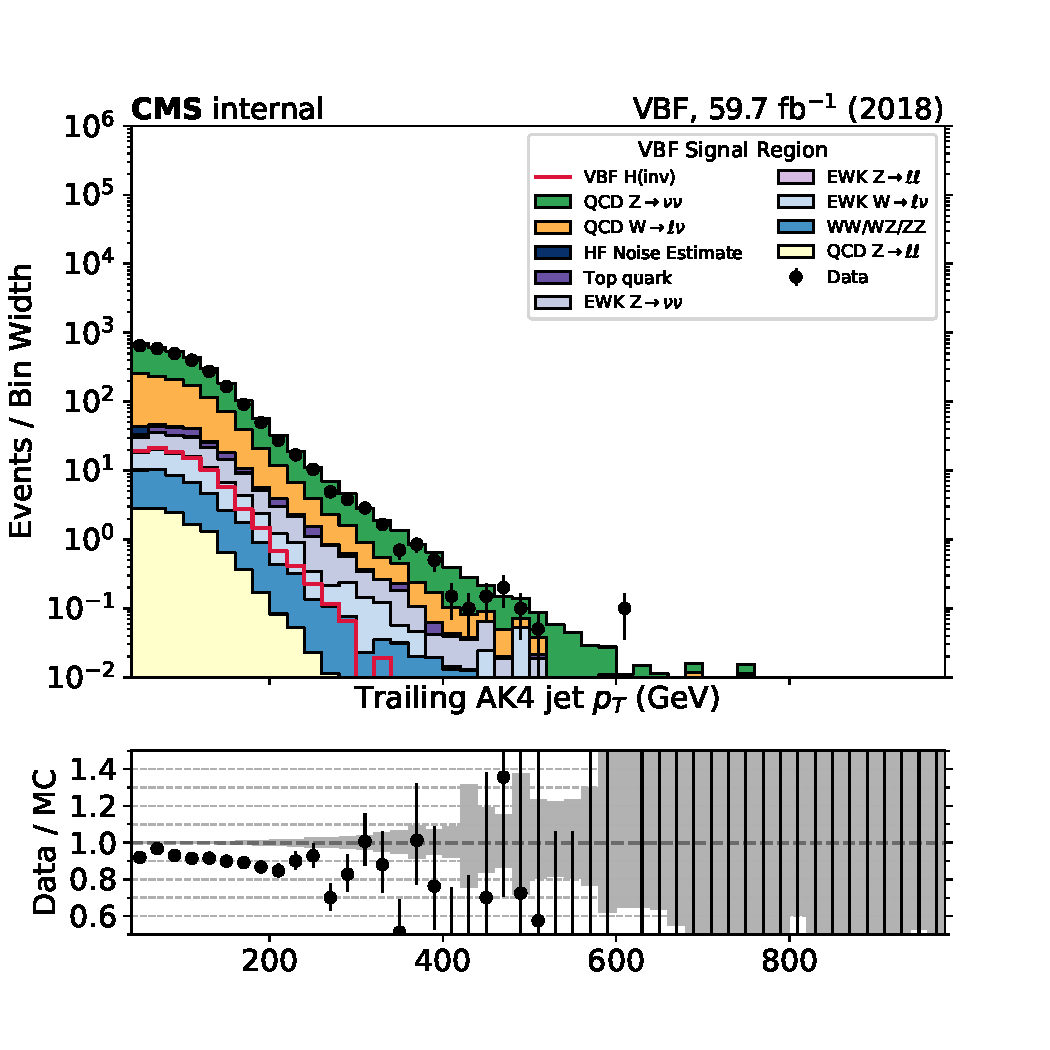
\includegraphics[width=0.49\textwidth]{\plotDir/sr_vbf/sr_vbf_data_mc_ak4_pt1_2018.pdf}
    \end{center}
    \caption{Leading and subleading jets $\pt$ and $\eta$ in the VBF signal region, using 2018 dataset.}
    \label{fig:SR_jets_vbfhinv_2018_mtr}
\end{figure}

\begin{figure}[htbp]
    \begin{center}
        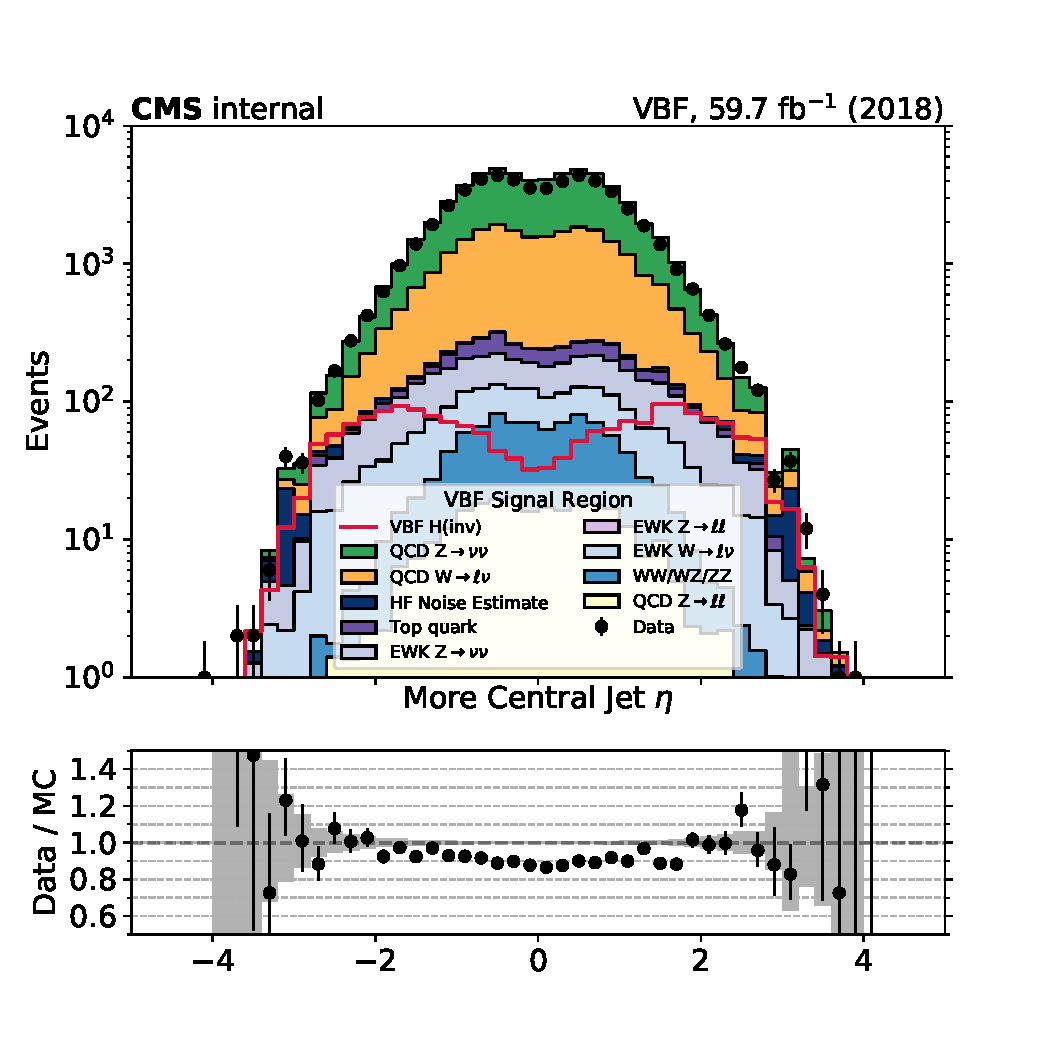
\includegraphics[width=0.49\textwidth]{\plotDir/sr_vbf/sr_vbf_data_mc_ak4_central_eta_2018.pdf}
        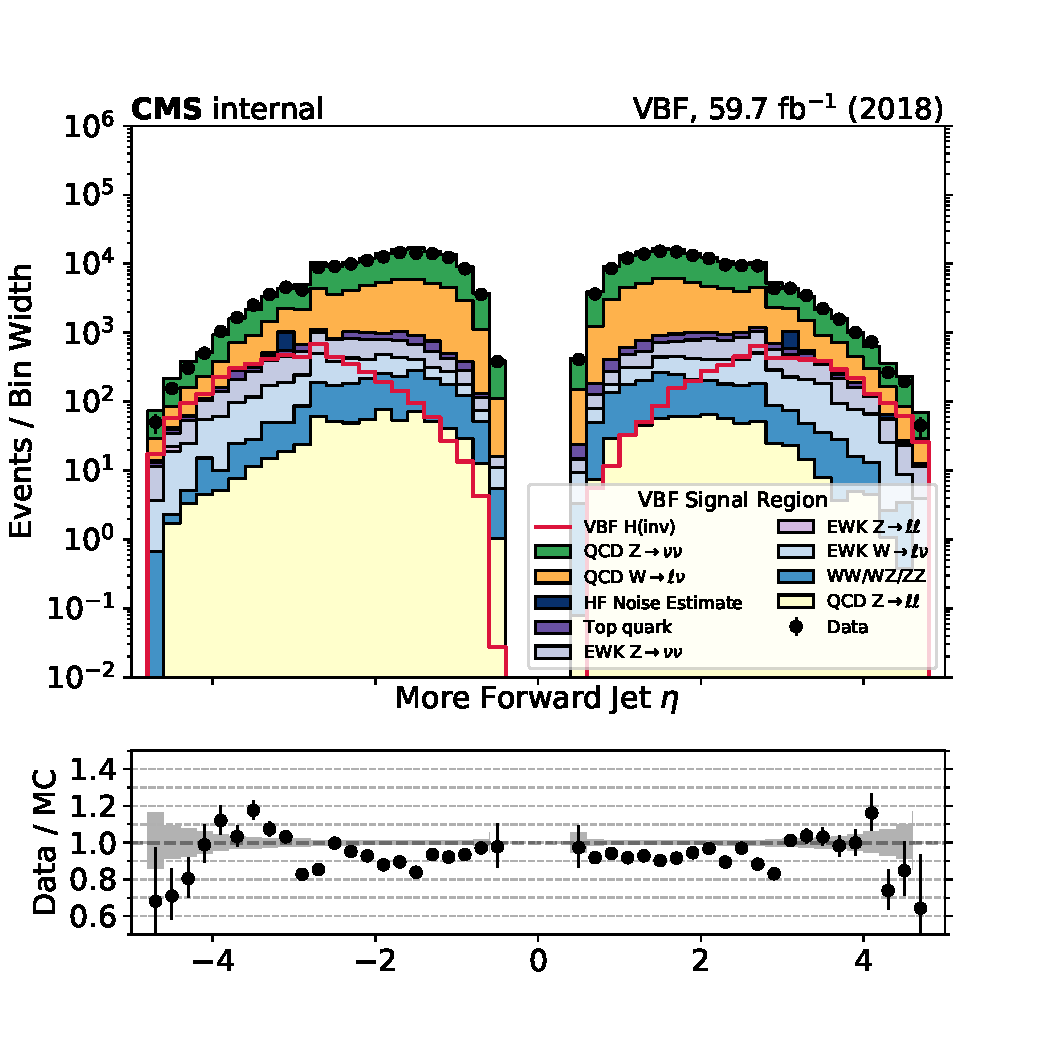
\includegraphics[width=0.49\textwidth]{\plotDir/sr_vbf/sr_vbf_data_mc_ak4_forward_eta_2018.pdf}
    \end{center}
    \caption{Most central (left) and most forward jets (right) $\eta$ of the VBF pair in the VBF signal region, using 2018 dataset.}
    \label{fig:SR_eta_vbfhinv_2018_mtr}
\end{figure}

% \begin{figure}[htbp]
%     \begin{center}
%         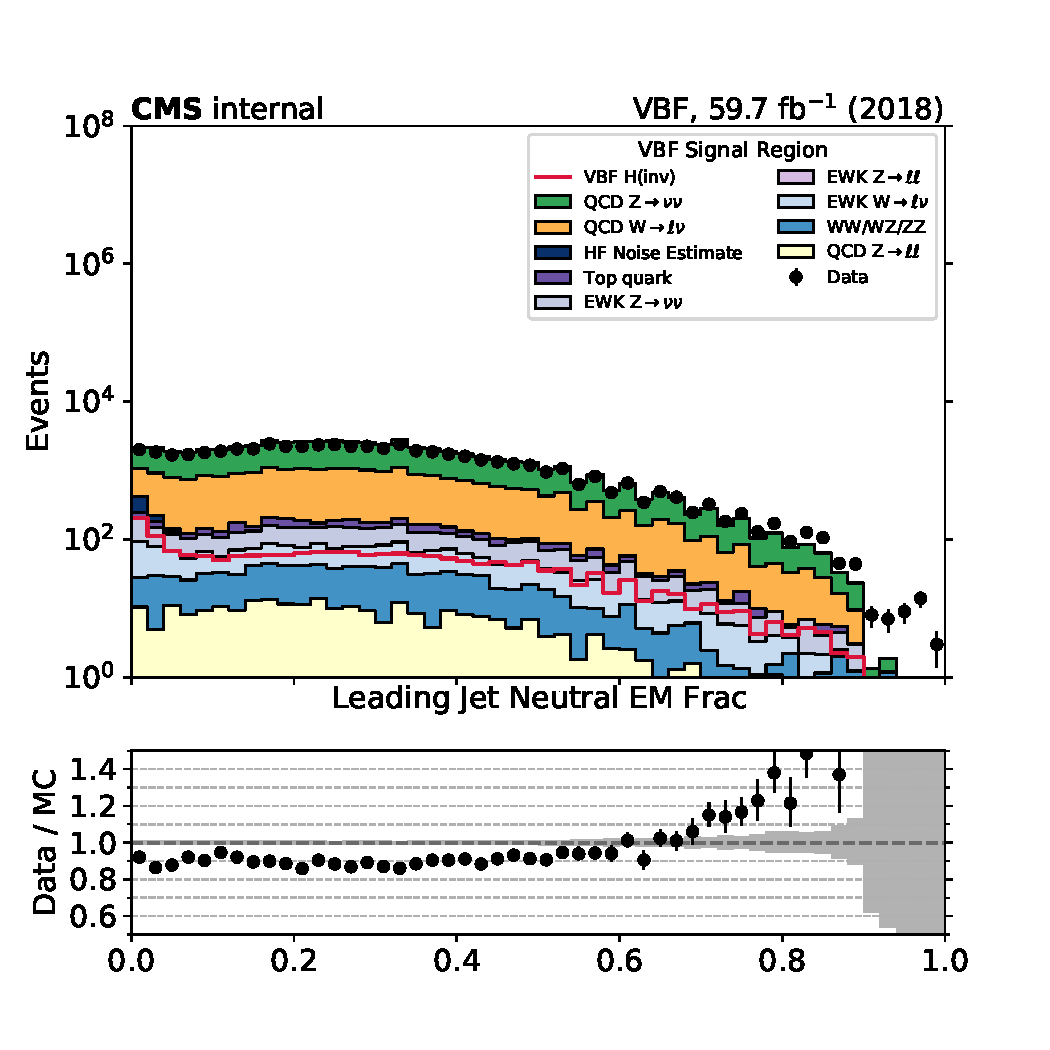
\includegraphics[width=0.49\textwidth]{\plotDir/sr_vbf/sr_vbf_data_mc_ak4_nef0_2018.pdf}
%         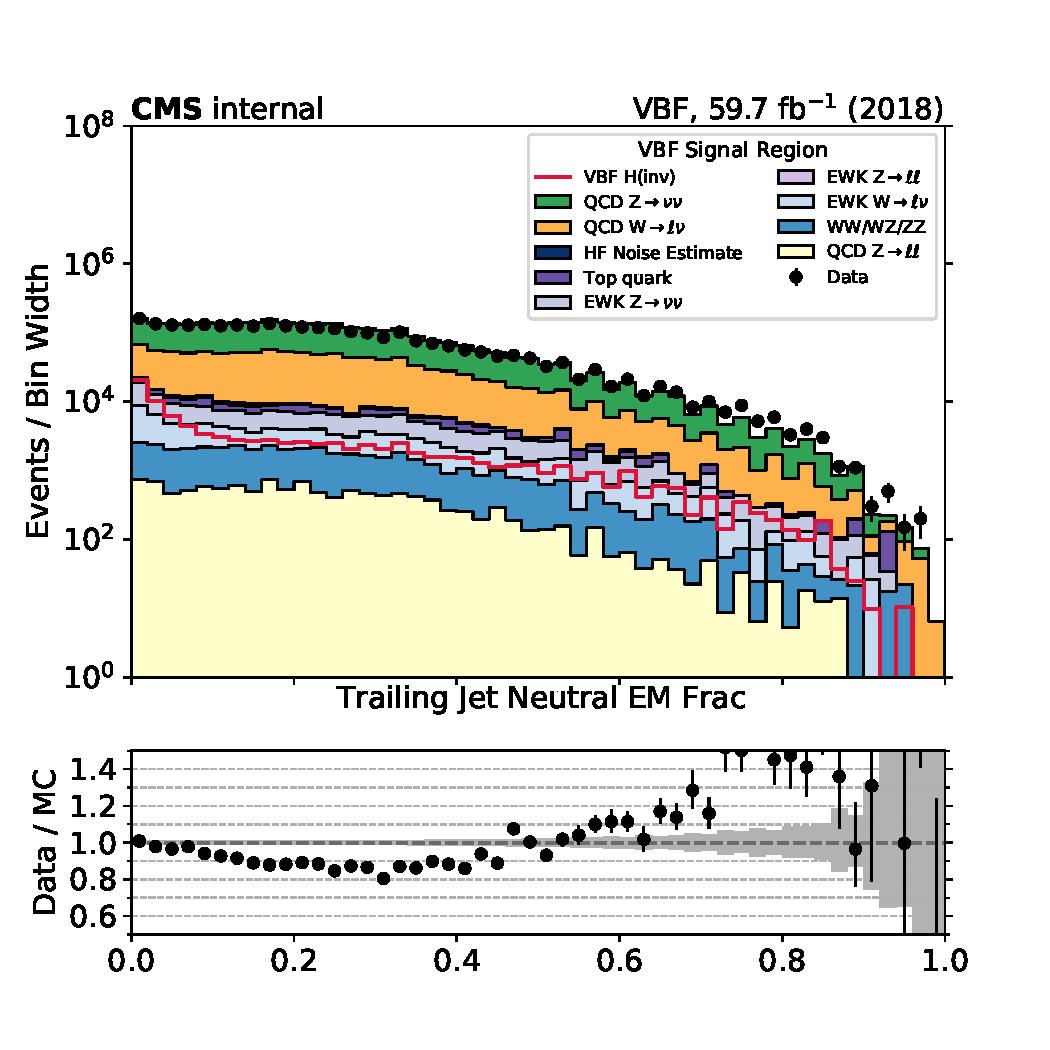
\includegraphics[width=0.49\textwidth]{\plotDir/sr_vbf/sr_vbf_data_mc_ak4_nef1_2018.pdf} \\
%         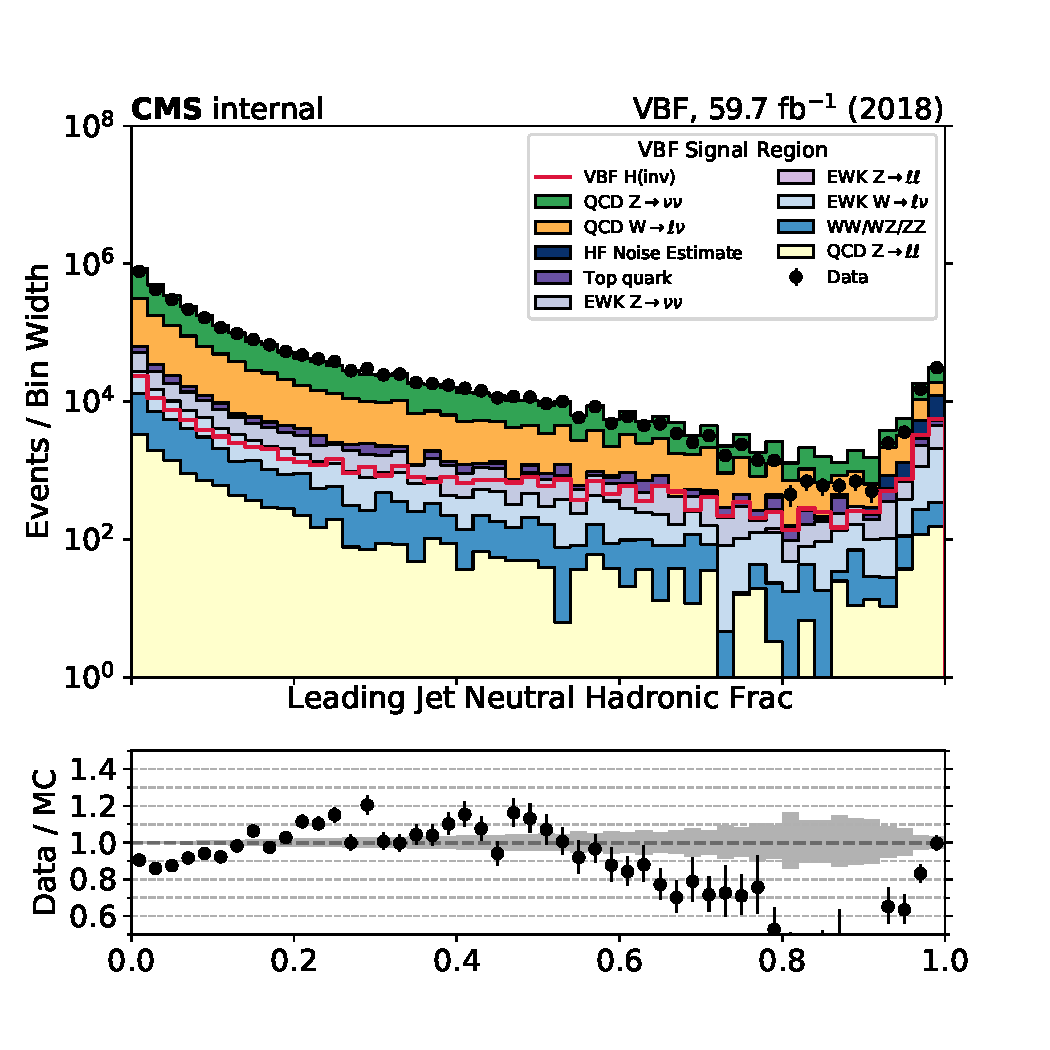
\includegraphics[width=0.49\textwidth]{\plotDir/sr_vbf/sr_vbf_data_mc_ak4_nhf0_2018.pdf}
%         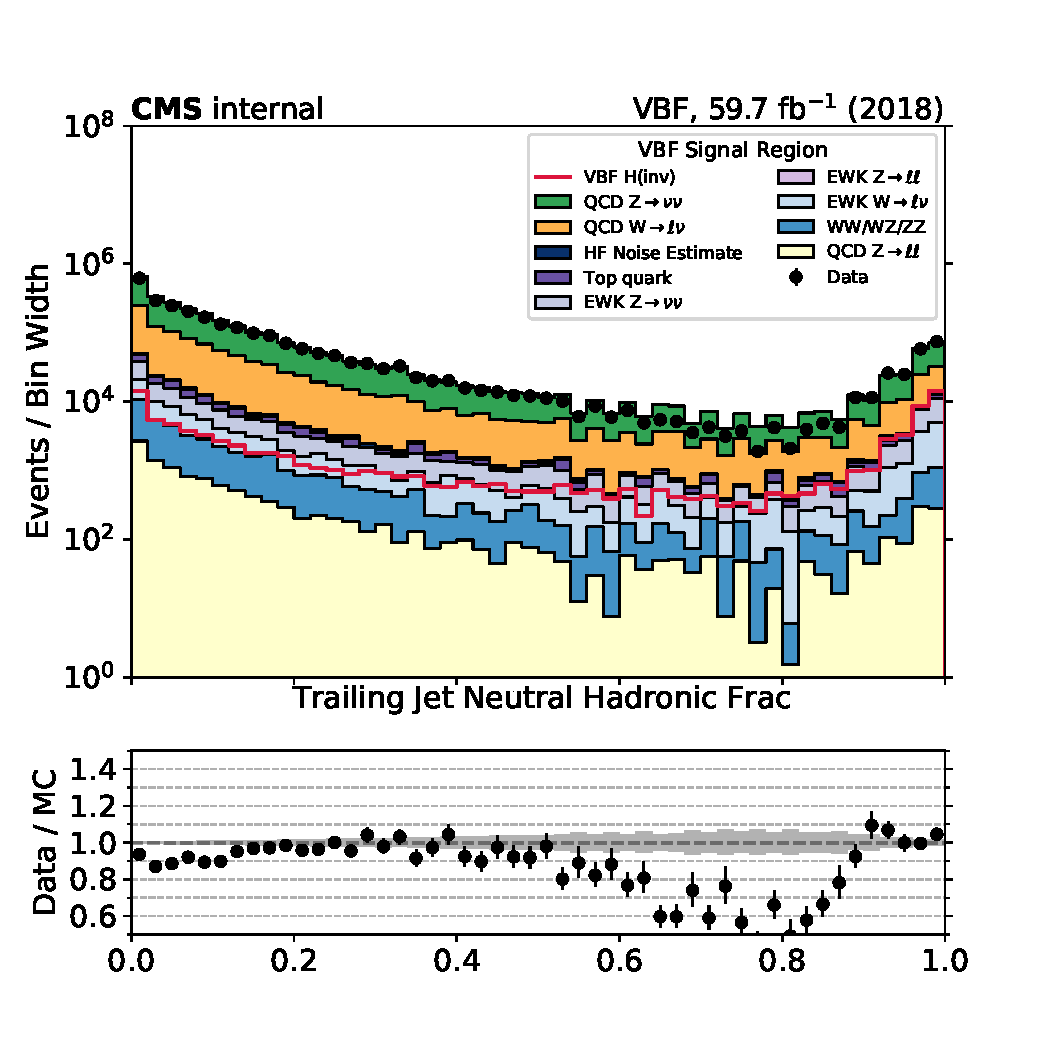
\includegraphics[width=0.49\textwidth]{\plotDir/sr_vbf/sr_vbf_data_mc_ak4_nhf1_2018.pdf} \\
%     \end{center}
%     \caption{Neutral electromagnetic energy fractions (top) and neutral hadron energy fractions for the leading two jets in the VBF signal region,
%     using 2018 dataset.}
%     \label{fig:SR_nhf_nef_2018_mtr}
% \end{figure}


% \begin{figure}[htbp]
%     \begin{center}
%         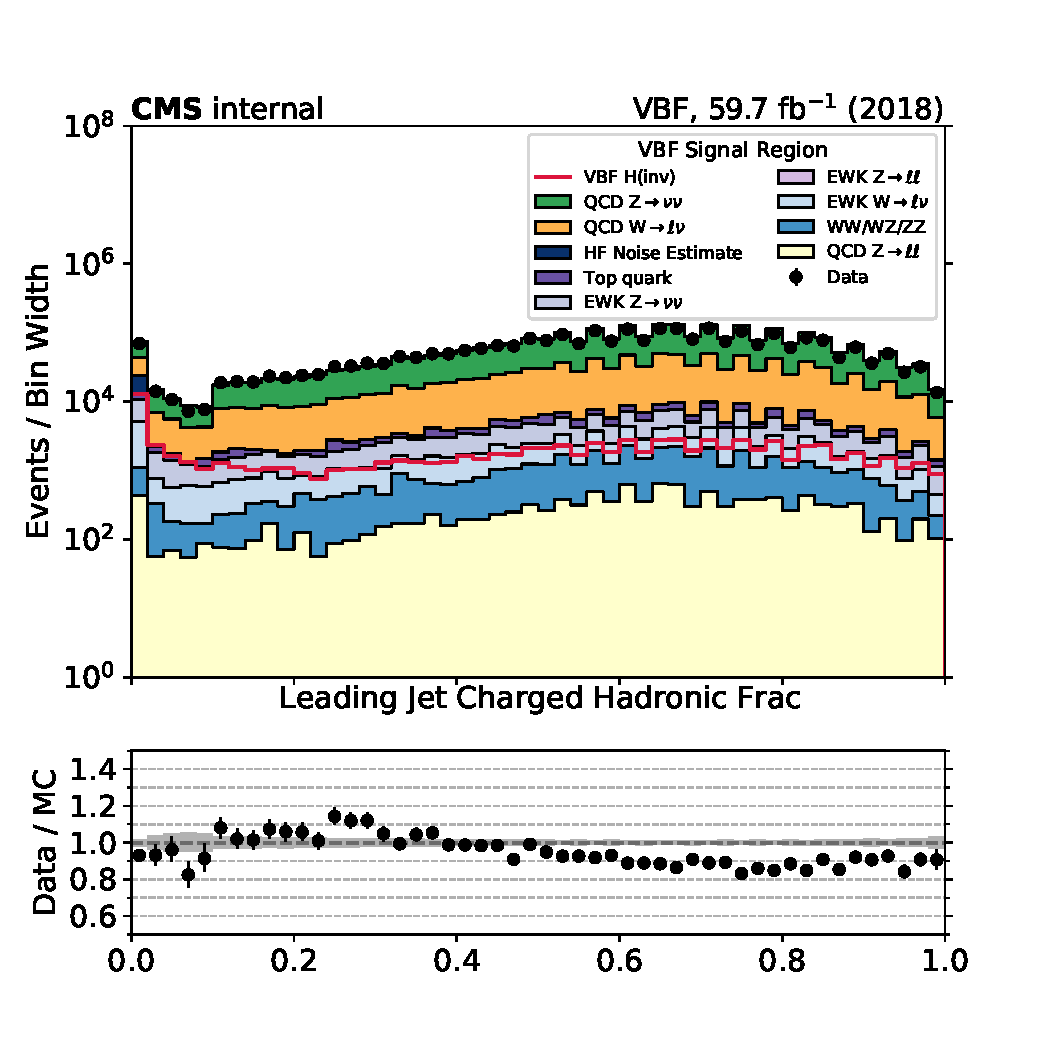
\includegraphics[width=0.49\textwidth]{\plotDir/sr_vbf/sr_vbf_data_mc_ak4_chf0_2018.pdf}
%         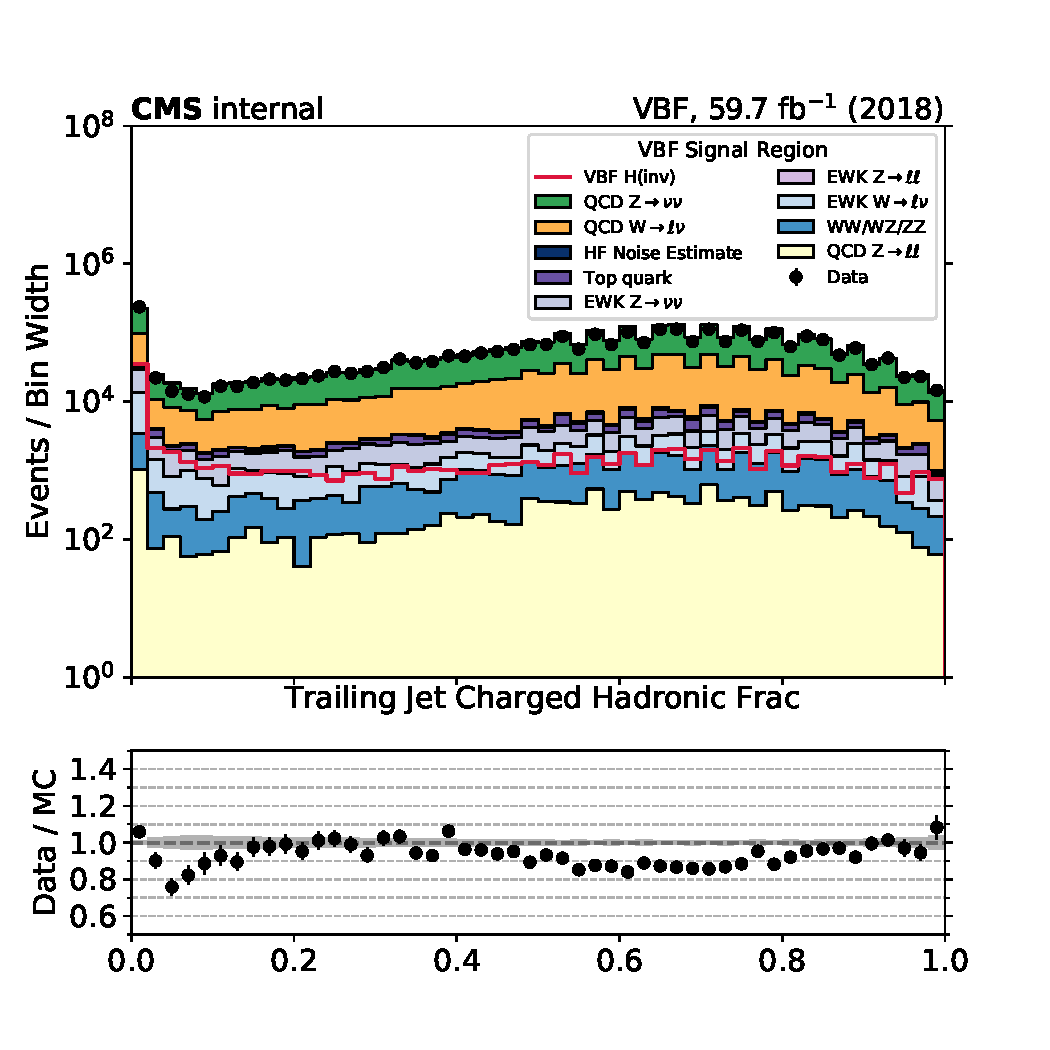
\includegraphics[width=0.49\textwidth]{\plotDir/sr_vbf/sr_vbf_data_mc_ak4_chf1_2018.pdf}
%     \end{center}
%     \caption{Charged hadronic energy fractions for the leading two jets in the VBF signal region,
%     using 2018 dataset.}
%     \label{fig:SR_chf_2018_mtr}
% \end{figure}

\clearpage

\subsection{Single Muon Control Region}
\label{sec:selection_cr_1m}

Single-muon control-region events are selected using full signal-region criteria of VBF selection with the exception of the muon veto. 
The \ptmiss requirement is replaced by an identical requirement on the hadronic recoil, which is defined as the sum of \ptvecmiss and the muon \vpt (Eq.~\ref{eq:recoil_def}), 
and thus corresponds to the \pt of the W boson.
In the single-muon control region, exactly one tightly identified, isolated muon with $\pt > 20$ GeV is required. 
No additional loose muons or electrons with $\pt > 10$ GeV are allowed in the event.

Figs.~\ref{fig:cr_1m_vbf_2017_mtr} and~\ref{fig:cr_1m_vbf_2018_mtr} show the distributions of $\mjj$, $\detajj$ for the two VBF jets,
and the $\pt$ and $\eta$ of the muon, the decay product of the $W$ boson, for 2017 and 2018 datasets respectively.

\begin{figure}[htbp]
    \begin{center}
        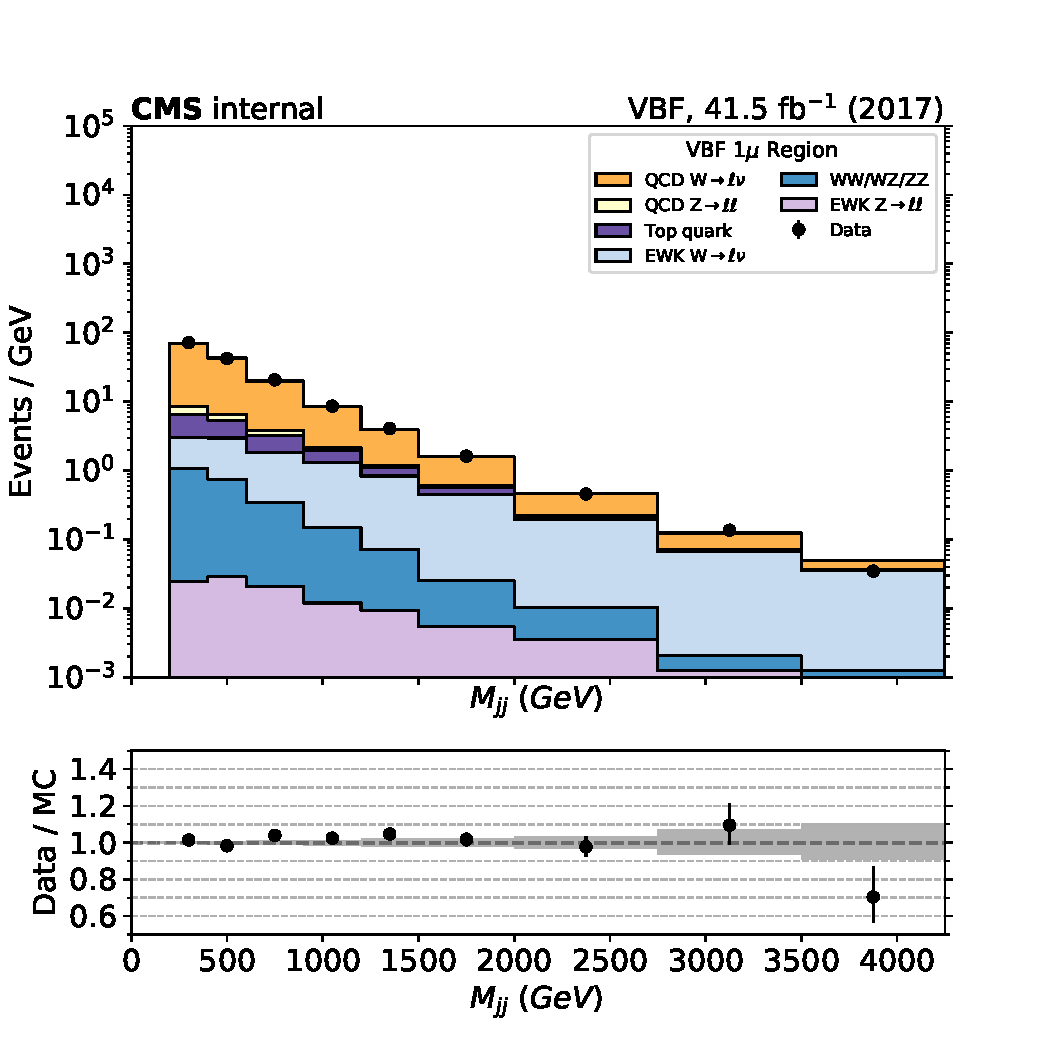
\includegraphics[width=0.49\textwidth]{\plotDir/cr_1m_vbf/cr_1m_vbf_data_mc_mjj_2017.pdf}
        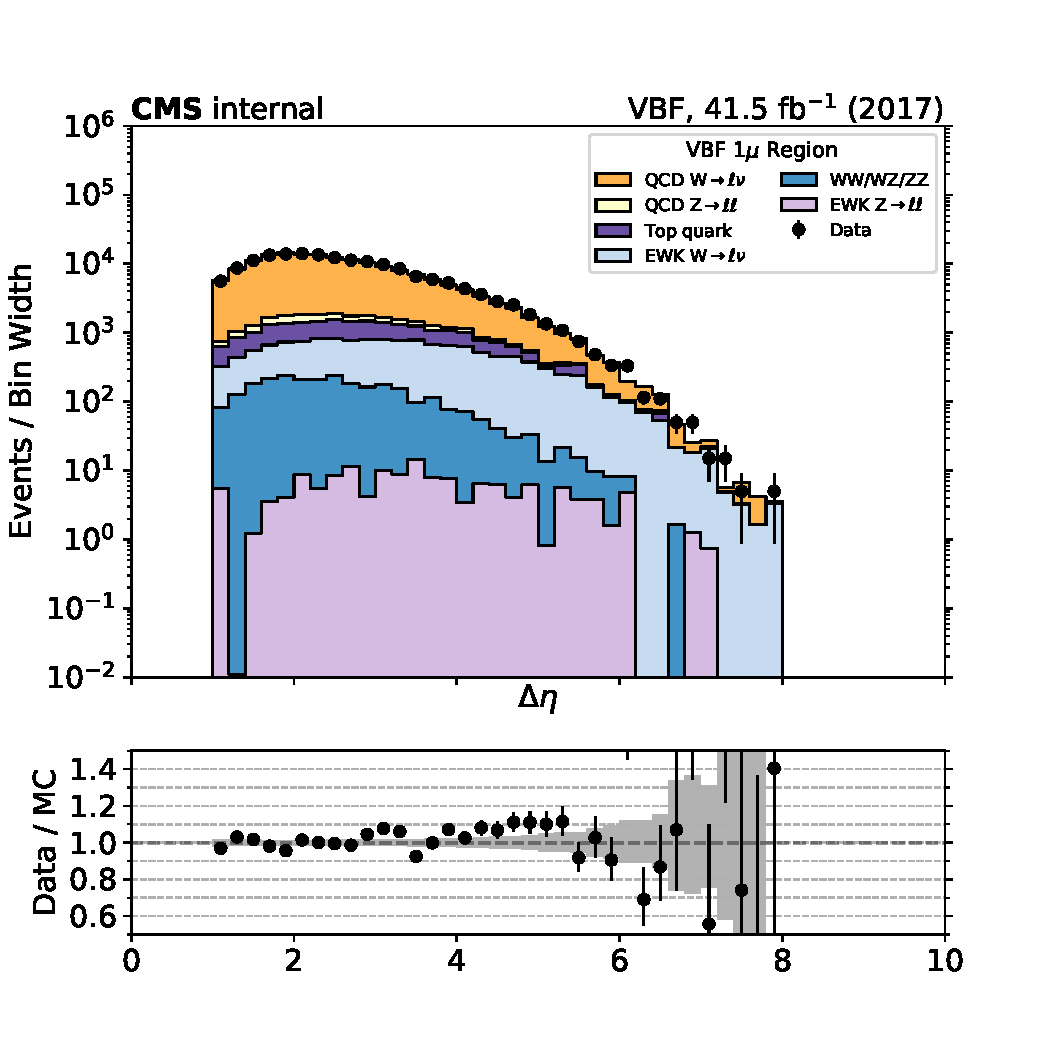
\includegraphics[width=0.49\textwidth]{\plotDir/cr_1m_vbf/cr_1m_vbf_data_mc_detajj_2017.pdf} \\
        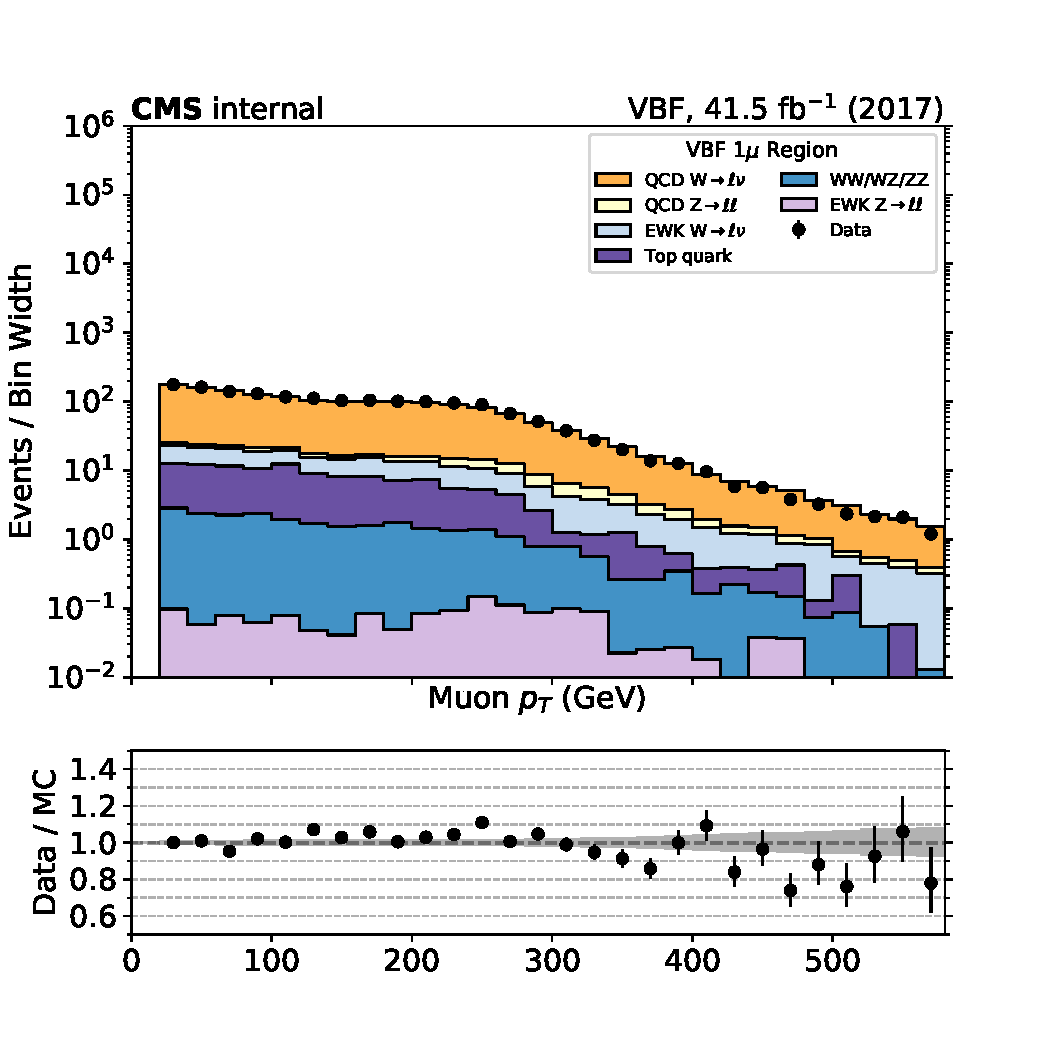
\includegraphics[width=0.49\textwidth]{\plotDir/cr_1m_vbf/cr_1m_vbf_data_mc_muon_pt_2017.pdf}
        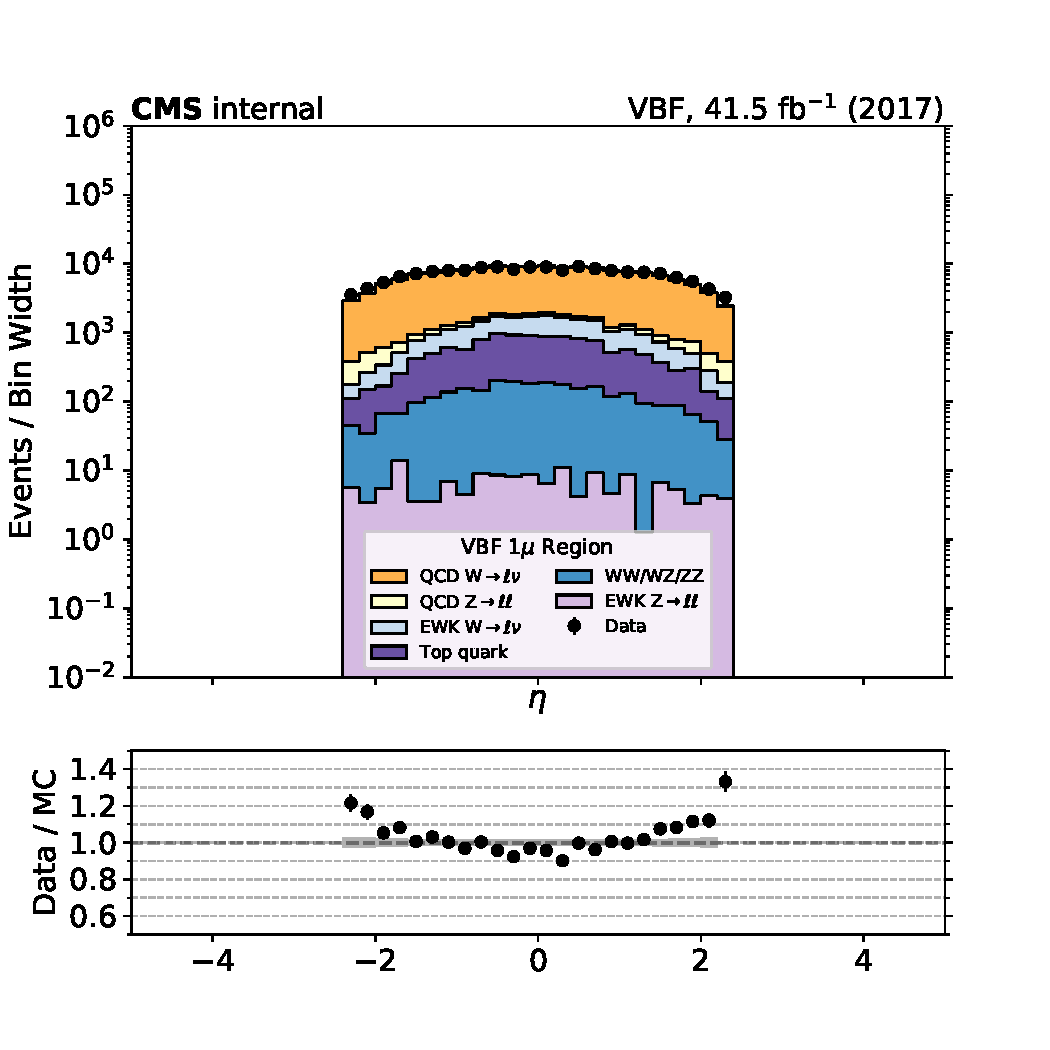
\includegraphics[width=0.49\textwidth]{\plotDir/cr_1m_vbf/cr_1m_vbf_data_mc_muon_eta_2017.pdf}
    \end{center}
    \caption{Comparison between 2017 data and Monte Carlo simulation in the single muon control region. Top plots
        show the $\mjj$ and $\detajj$ distributions for the two leading AK4 jets. Bottom plots show the $\pt$ and $\eta$
        of the reconstructed muon.}
    \label{fig:cr_1m_vbf_2017_mtr}
\end{figure}

\begin{figure}[htbp]
    \begin{center}
        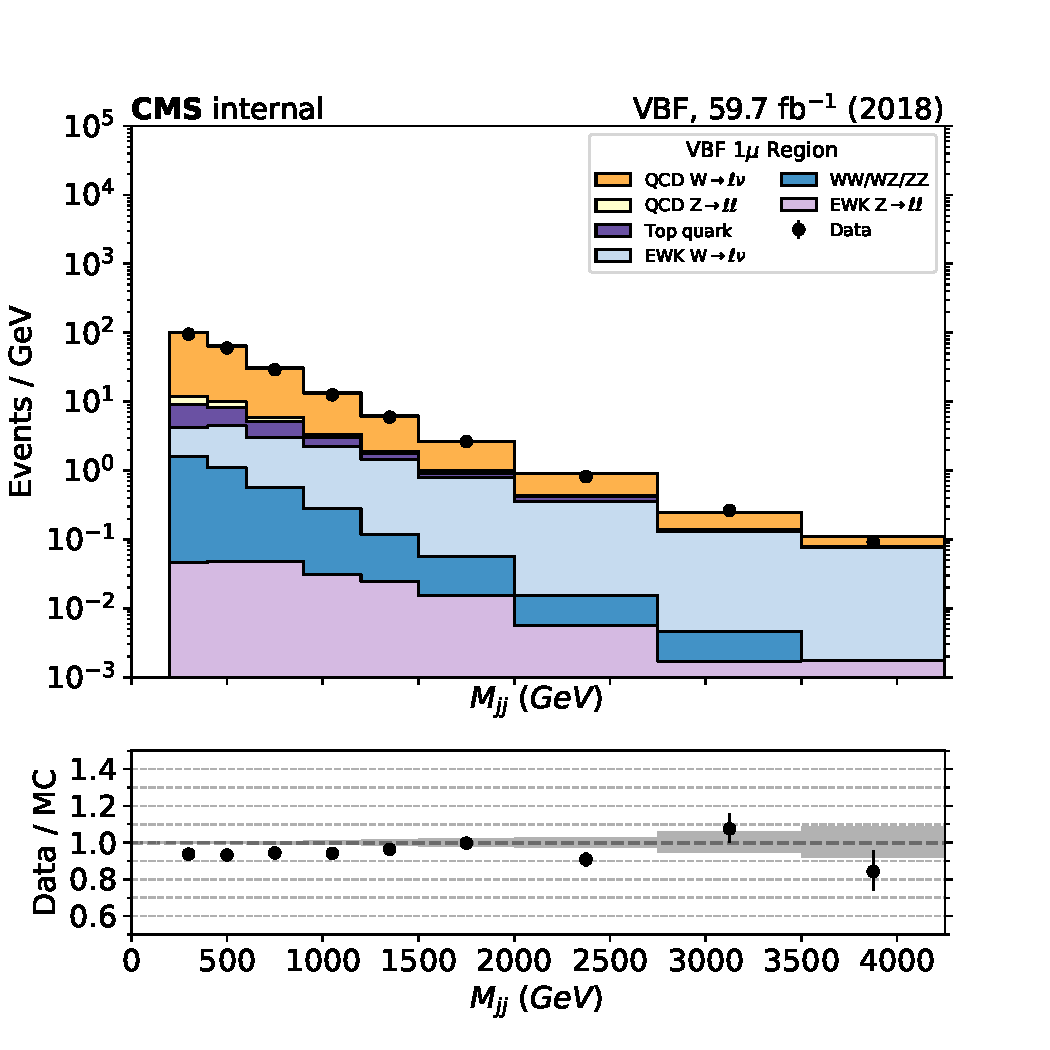
\includegraphics[width=0.49\textwidth]{\plotDir/cr_1m_vbf/cr_1m_vbf_data_mc_mjj_2018.pdf}
        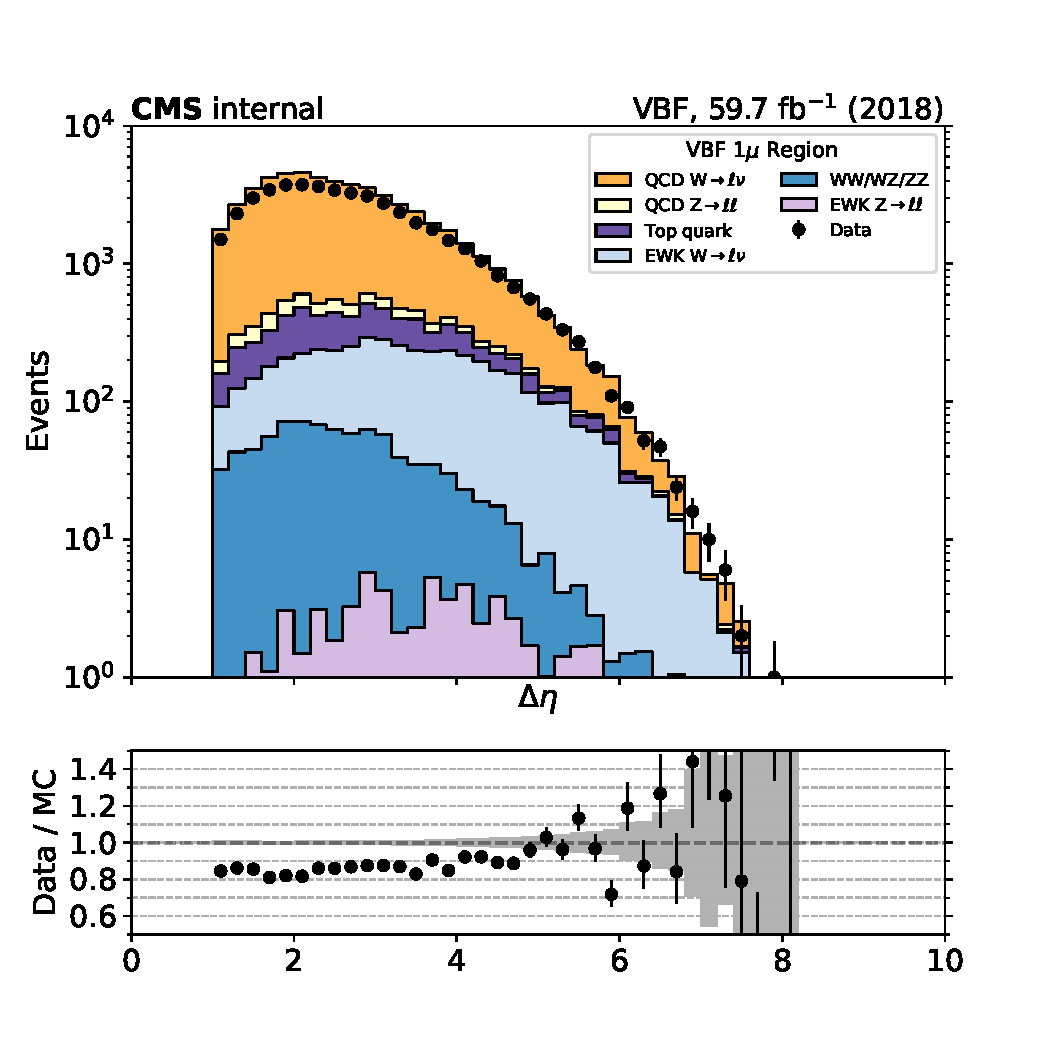
\includegraphics[width=0.49\textwidth]{\plotDir/cr_1m_vbf/cr_1m_vbf_data_mc_detajj_2018.pdf} \\
        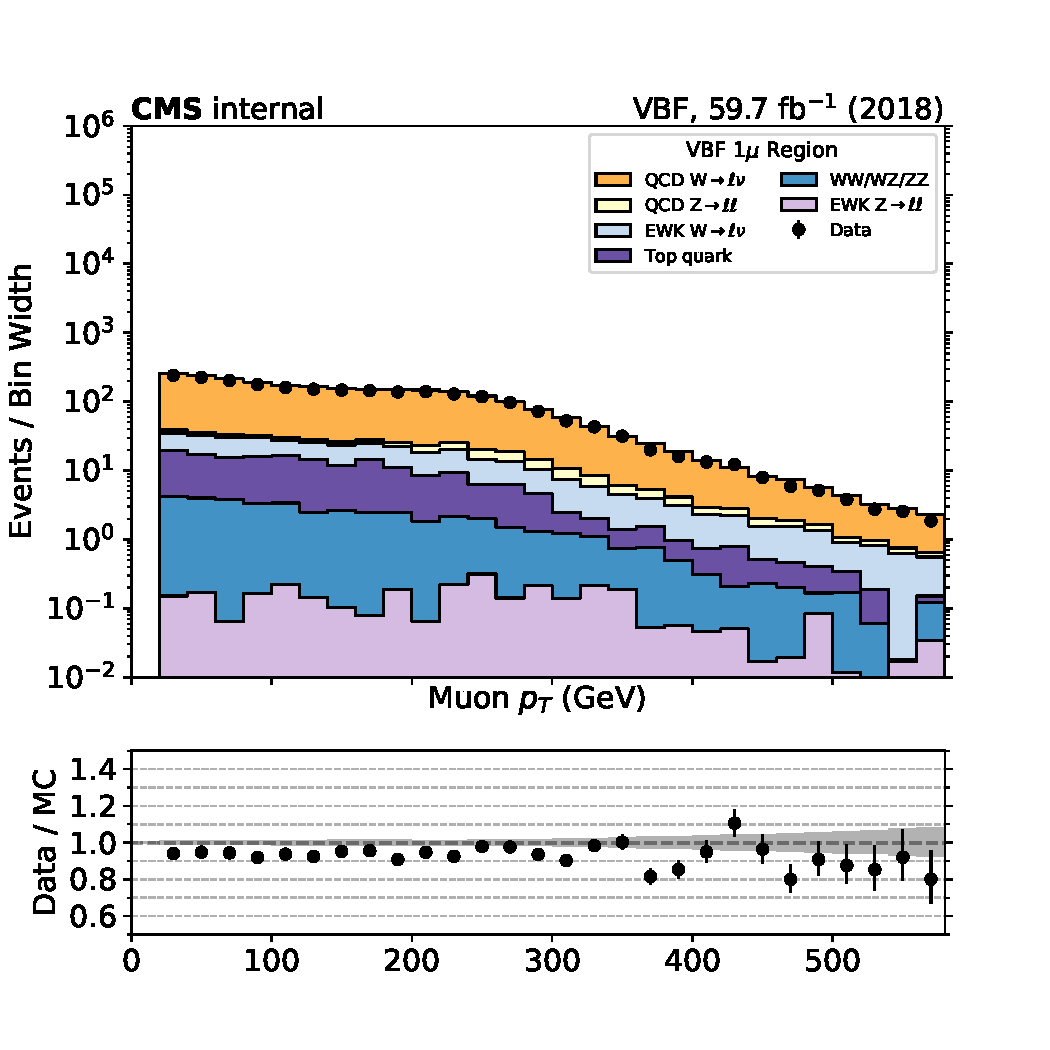
\includegraphics[width=0.49\textwidth]{\plotDir/cr_1m_vbf/cr_1m_vbf_data_mc_muon_pt_2018.pdf}
        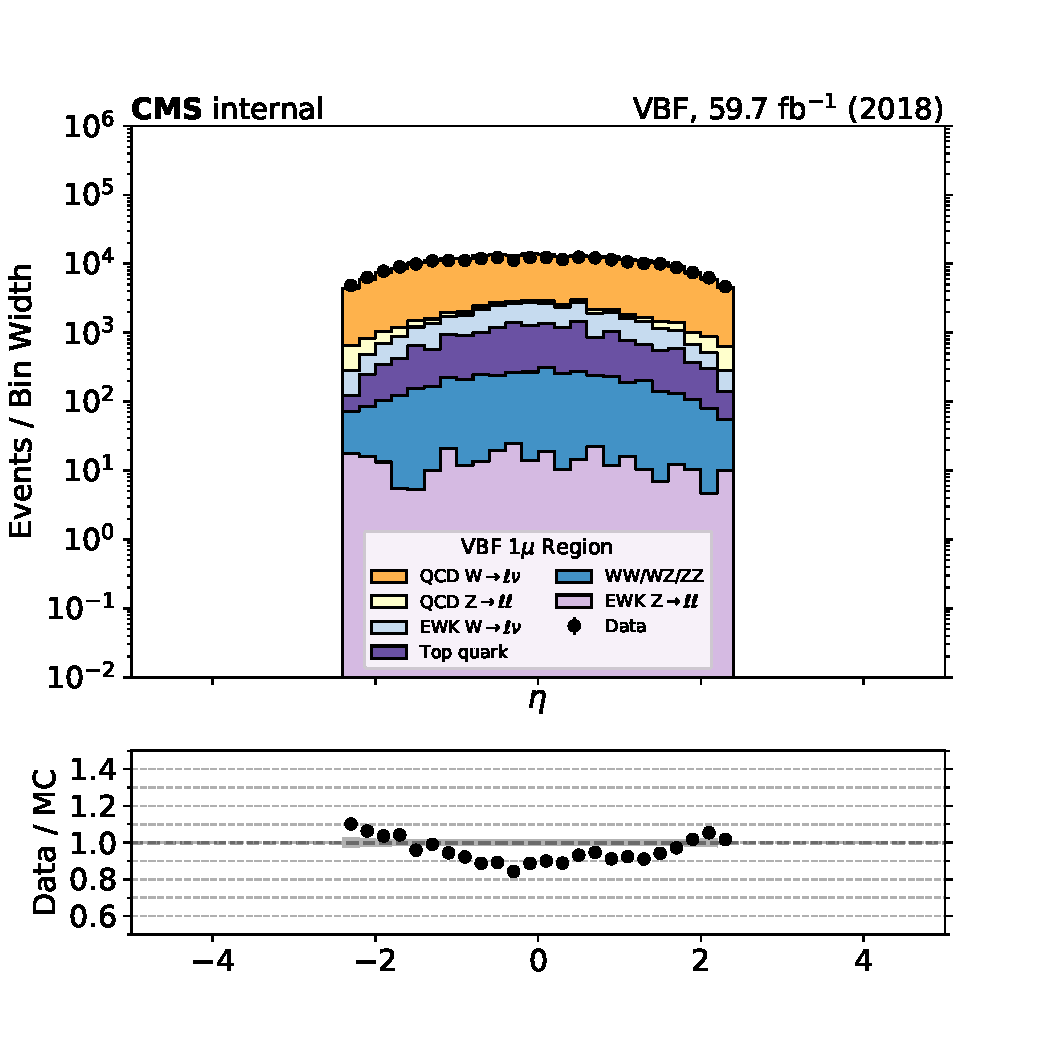
\includegraphics[width=0.49\textwidth]{\plotDir/cr_1m_vbf/cr_1m_vbf_data_mc_muon_eta_2018.pdf}
    \end{center}
    \caption{Comparison between 2018 data and Monte Carlo simulation in the single muon control region. Top plots
    show the $\mjj$ and $\detajj$ distributions for the two leading AK4 jets. Bottom plots show the $\pt$ and $\eta$
    of the reconstructed muon.}
    \label{fig:cr_1m_vbf_2018_mtr}
\end{figure}

\clearpage

\subsection{Single Electron Control Region}
\label{sec:selection_cr_1e}

Events for the single-electron control region are collected with the single-electron and photon triggers described in Sec.~\ref{subsec:trigger_eff_reweighting}.
Similar to the muon control regions, the \ptmiss requirement is replaced with an identical requirement on the hadronic recoil, which is defined as the sum of \ptvecmiss 
and the electron \vpt (Eq.~\ref{eq:recoil_def}), and thus corresponds to the \pt of the W boson.
The events in the single-electron control region are required to contain exactly one tightly identified and isolated electron with $\pt > 40$ GeV.
In addition, the contamination from QCD multijet events in this control region is suppressed by requiring $\ptmiss > 80$ GeV.

Figs.~\ref{fig:cr_1e_vbf_2017_mtr} and~\ref{fig:cr_1e_vbf_2018_mtr} show the distributions of $\mjj$, $\detajj$ for the two VBF jets,
and the $\pt$ and $\eta$ of the electron, the decay product of the $W$ boson, for 2017 and 2018 datasets respectively.

\begin{figure}[htbp]
    \begin{center}
        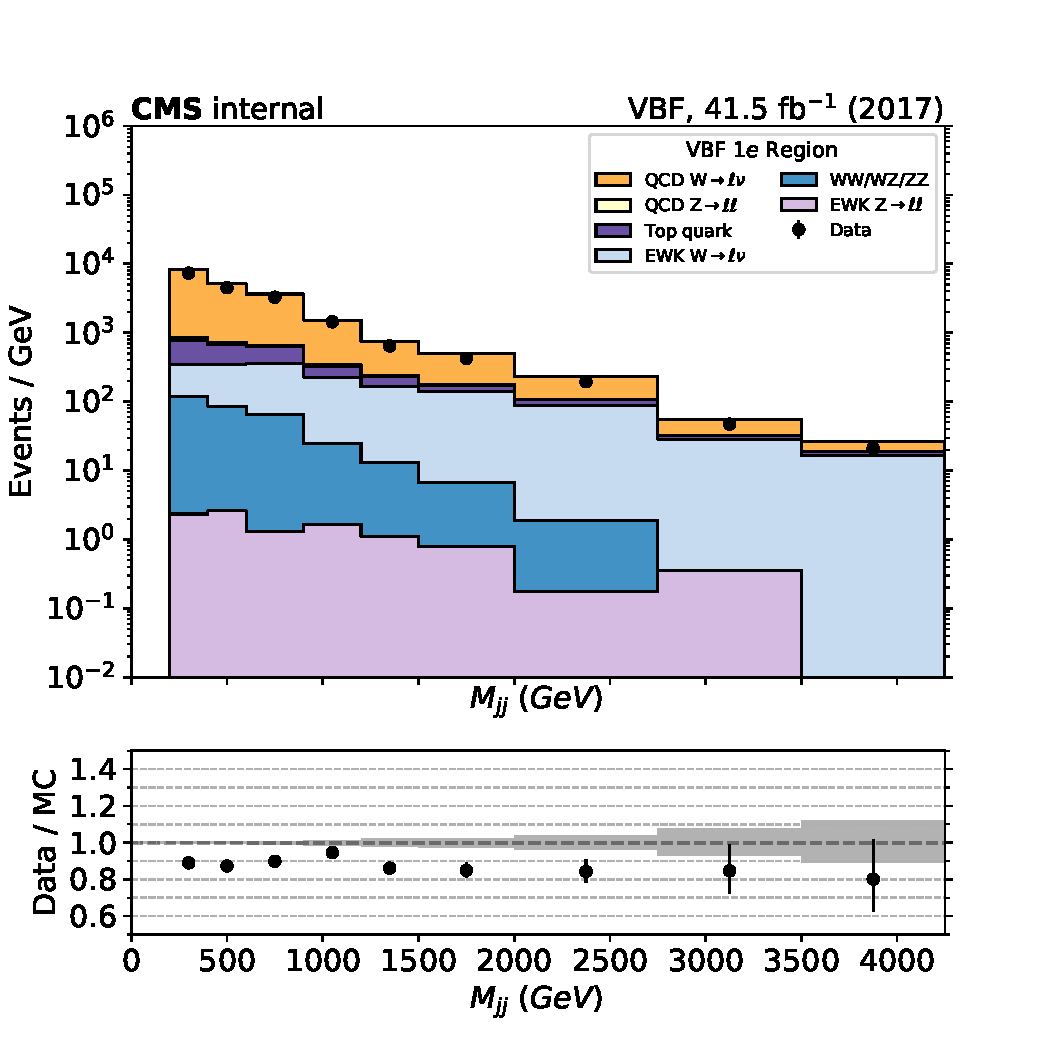
\includegraphics[width=0.49\textwidth]{\plotDir/cr_1e_vbf/cr_1e_vbf_data_mc_mjj_2017.pdf}
        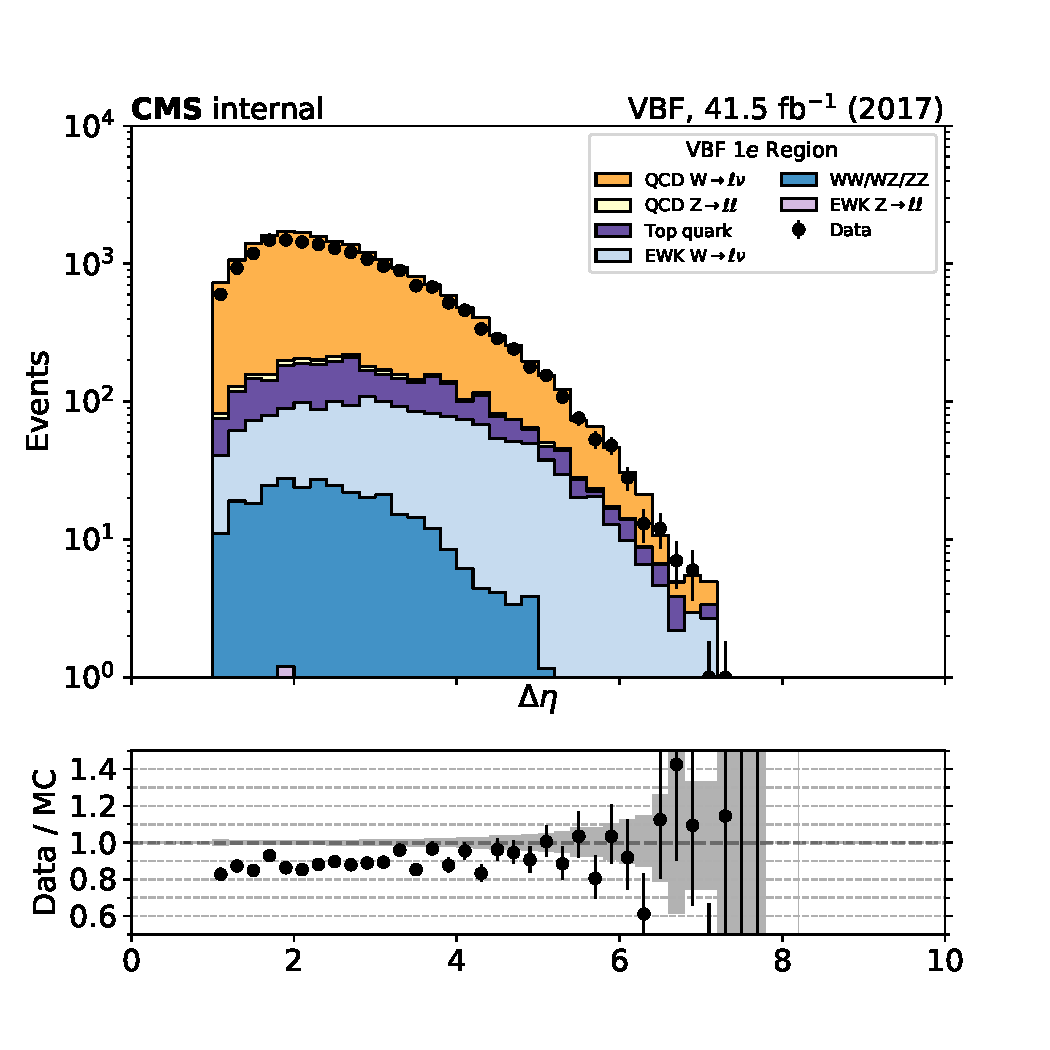
\includegraphics[width=0.49\textwidth]{\plotDir/cr_1e_vbf/cr_1e_vbf_data_mc_detajj_2017.pdf} \\
        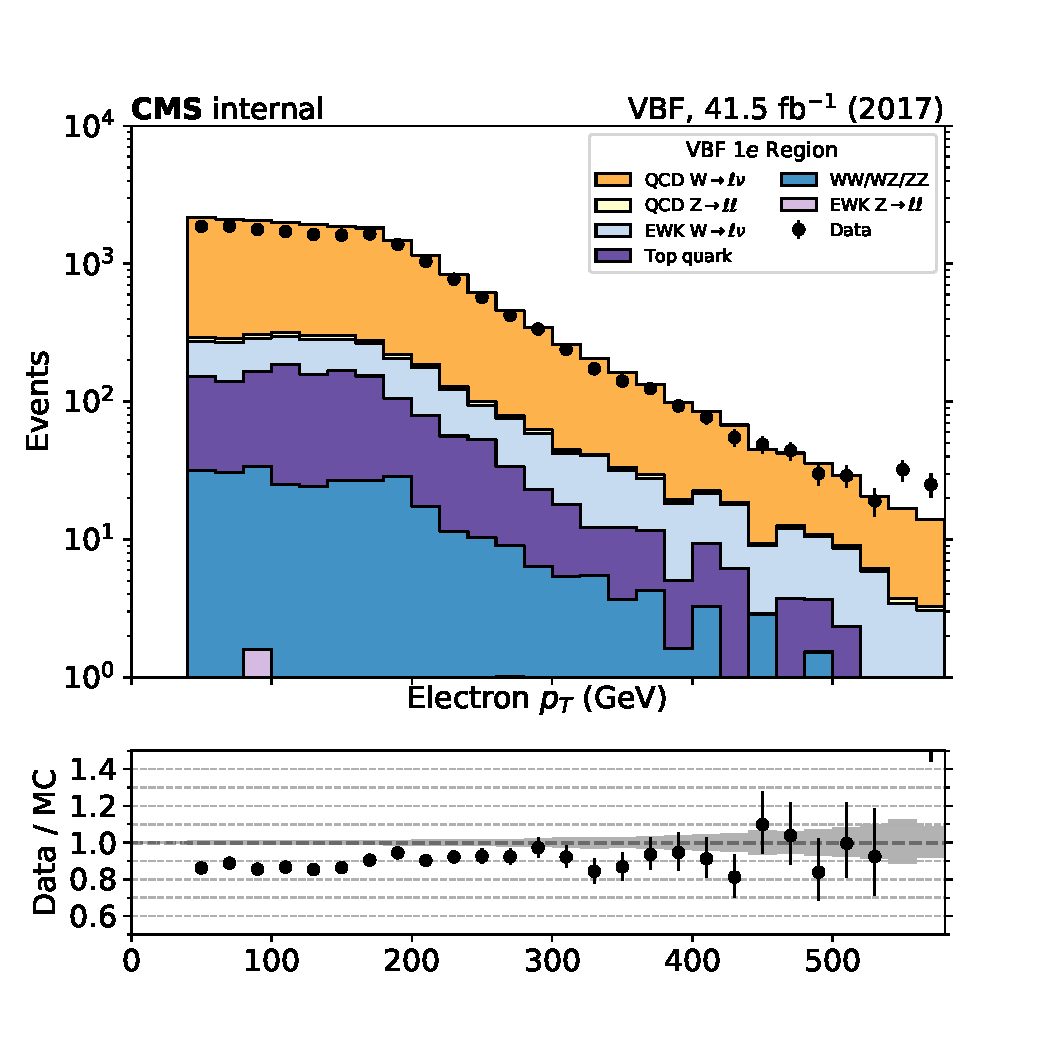
\includegraphics[width=0.49\textwidth]{\plotDir/cr_1e_vbf/cr_1e_vbf_data_mc_electron_pt_2017.pdf}
        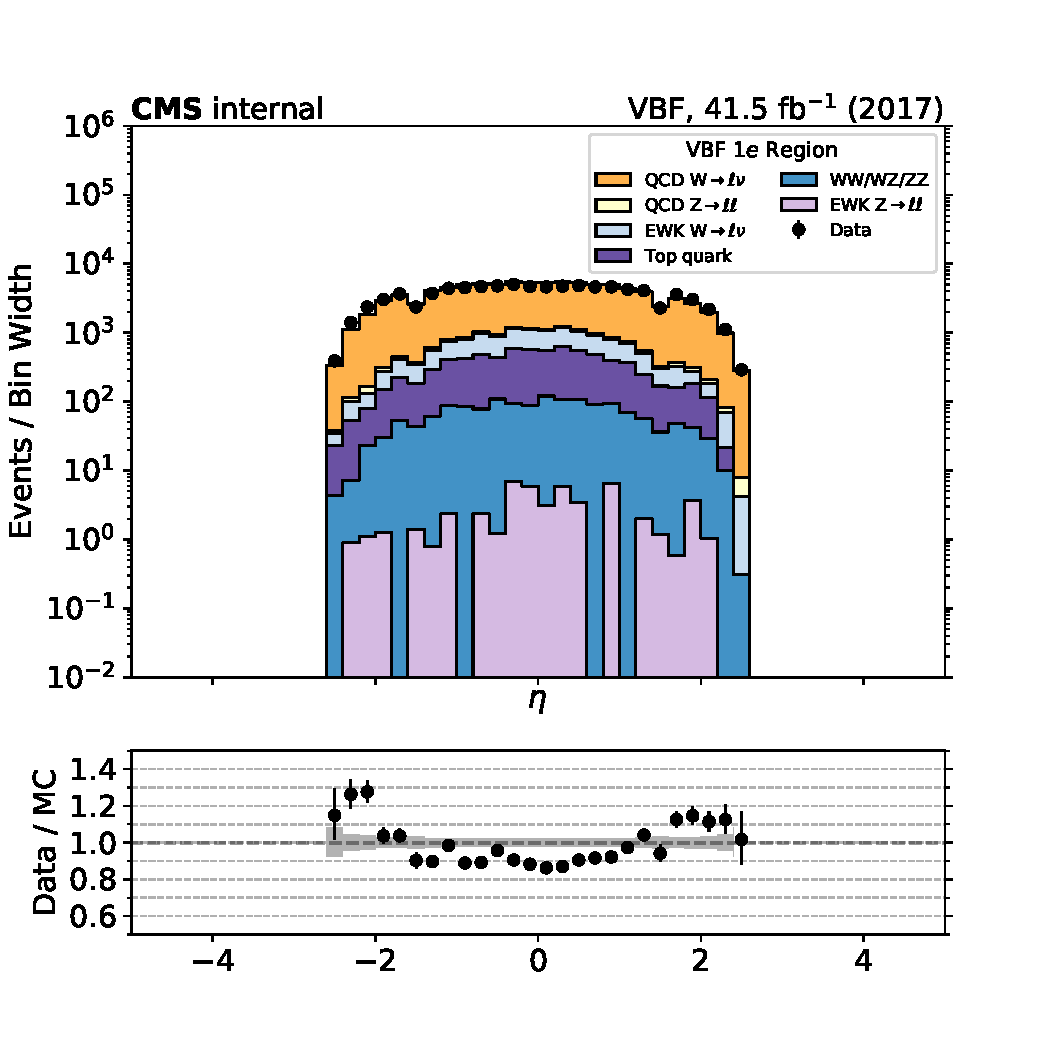
\includegraphics[width=0.49\textwidth]{\plotDir/cr_1e_vbf/cr_1e_vbf_data_mc_electron_eta_2017.pdf}
    \end{center}
    \caption{Comparison between 2017 data and Monte Carlo simulation in the single electron control region. Top plots
    show the $\mjj$ and $\detajj$ distributions for the two leading AK4 jets. Bottom plots show the $\pt$ and $\eta$
    of the reconstructed electron.}
    \label{fig:cr_1e_vbf_2017_mtr}
\end{figure}

\begin{figure}[htbp]
    \begin{center}
        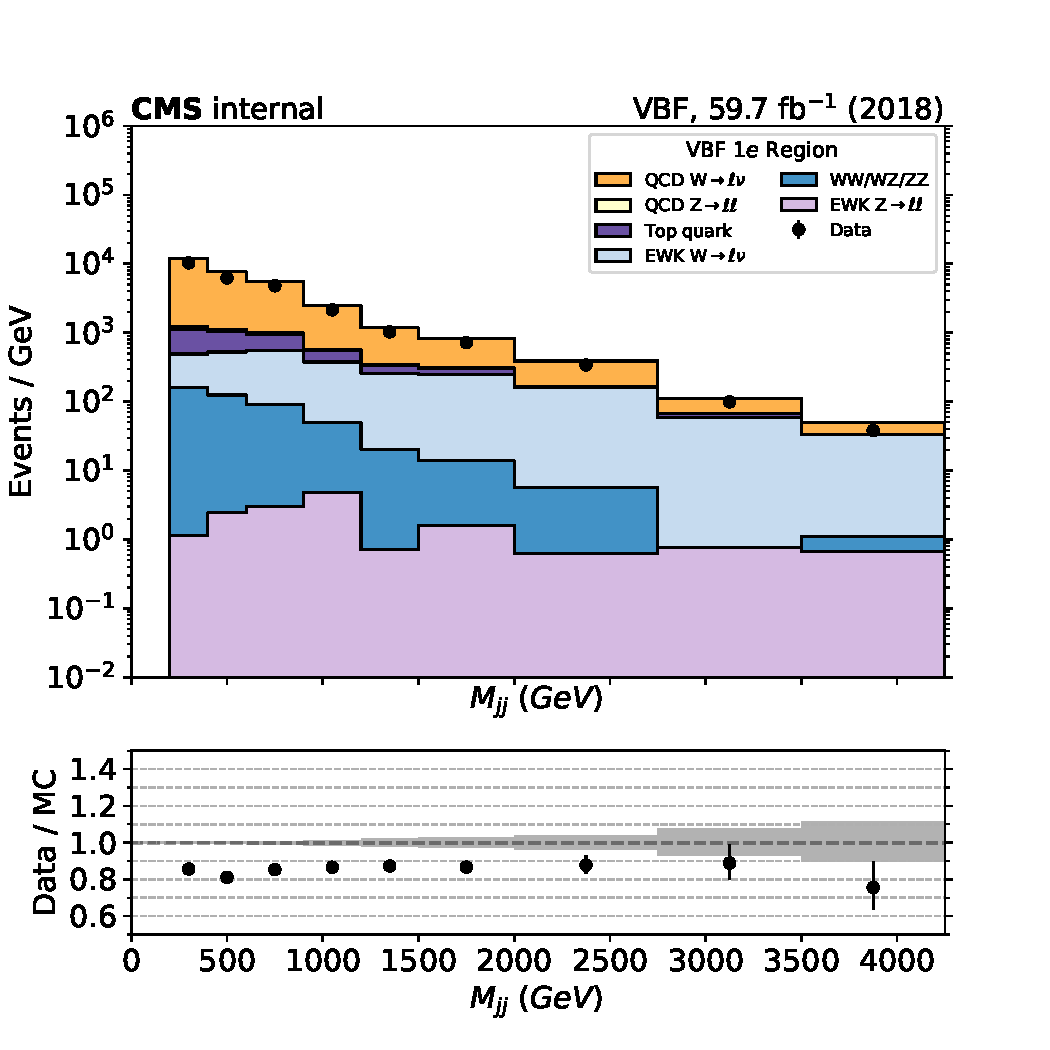
\includegraphics[width=0.49\textwidth]{\plotDir/cr_1e_vbf/cr_1e_vbf_data_mc_mjj_2018.pdf}
        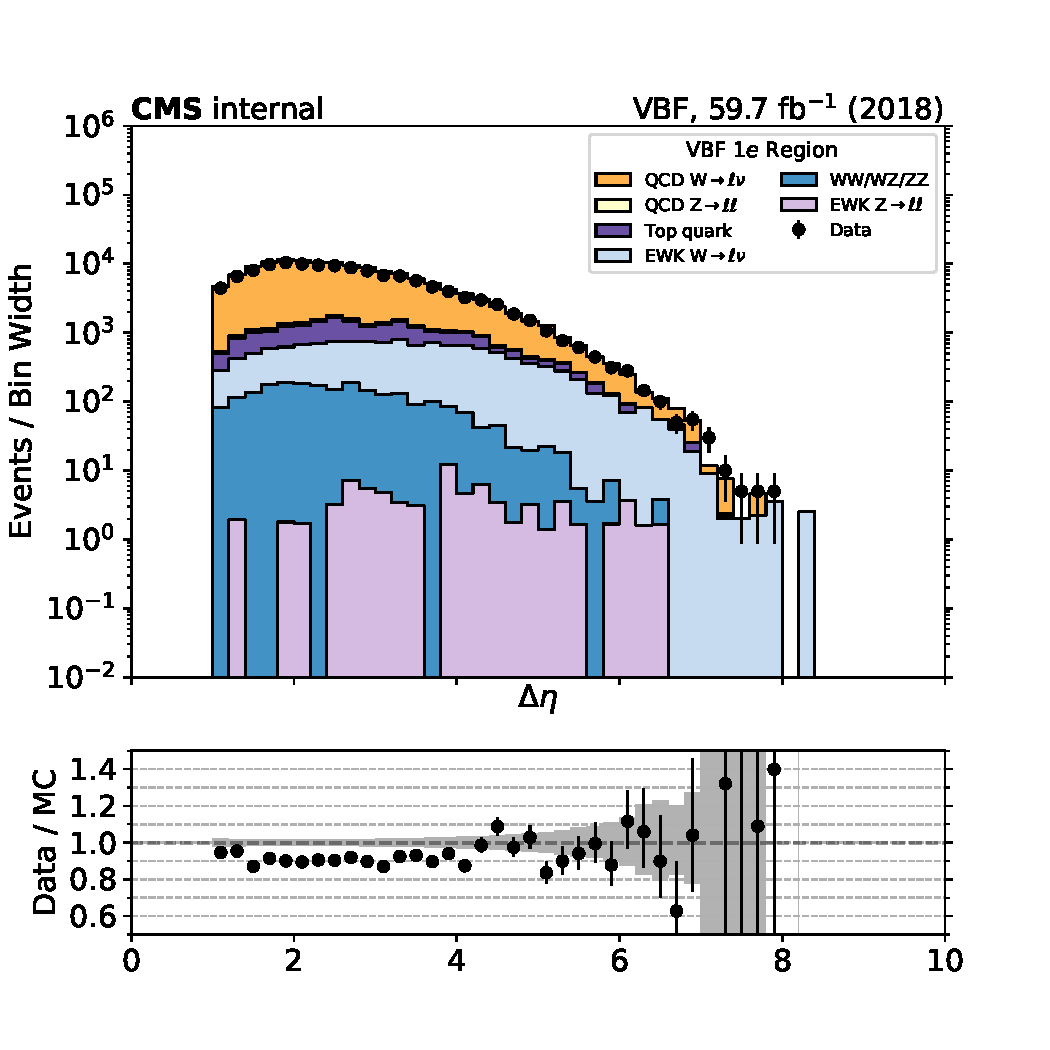
\includegraphics[width=0.49\textwidth]{\plotDir/cr_1e_vbf/cr_1e_vbf_data_mc_detajj_2018.pdf} \\
        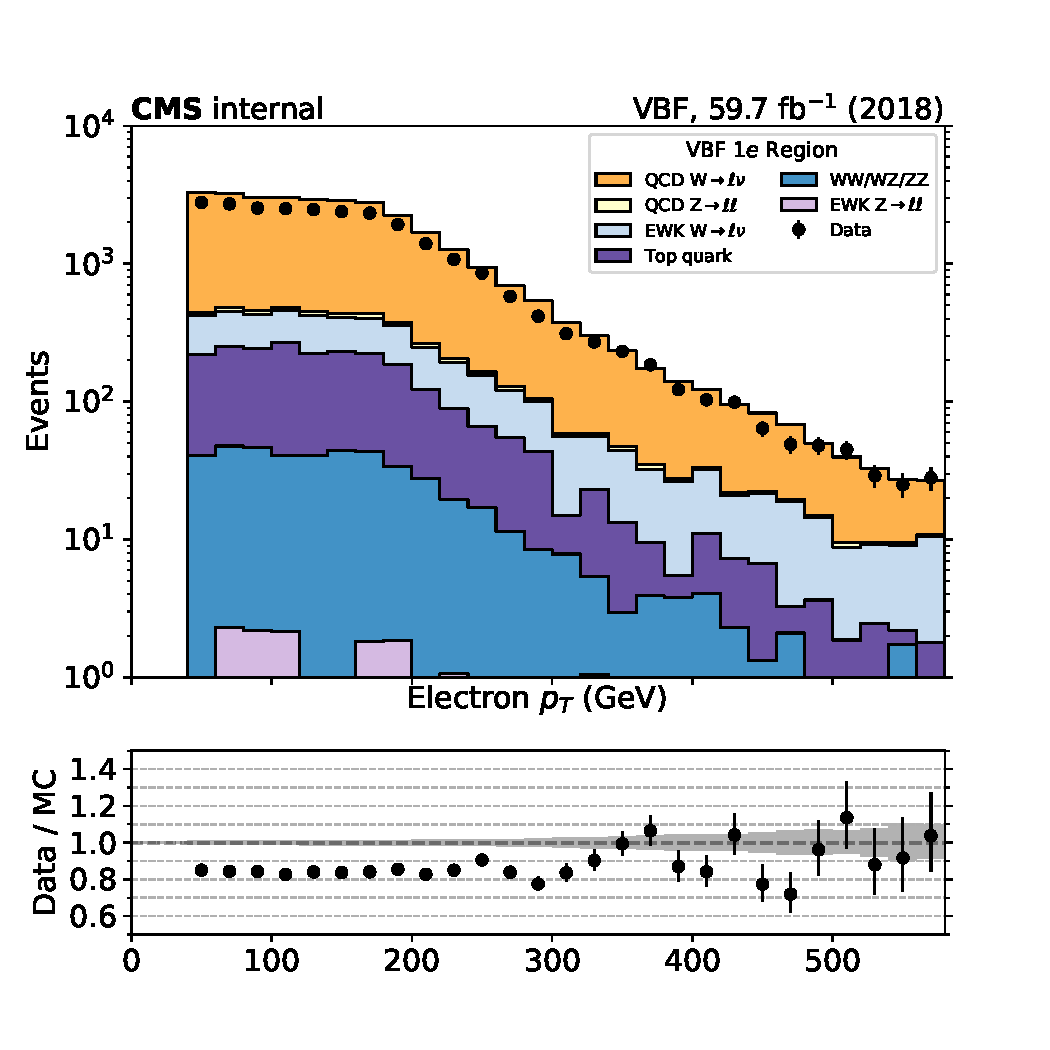
\includegraphics[width=0.49\textwidth]{\plotDir/cr_1e_vbf/cr_1e_vbf_data_mc_electron_pt_2018.pdf}
        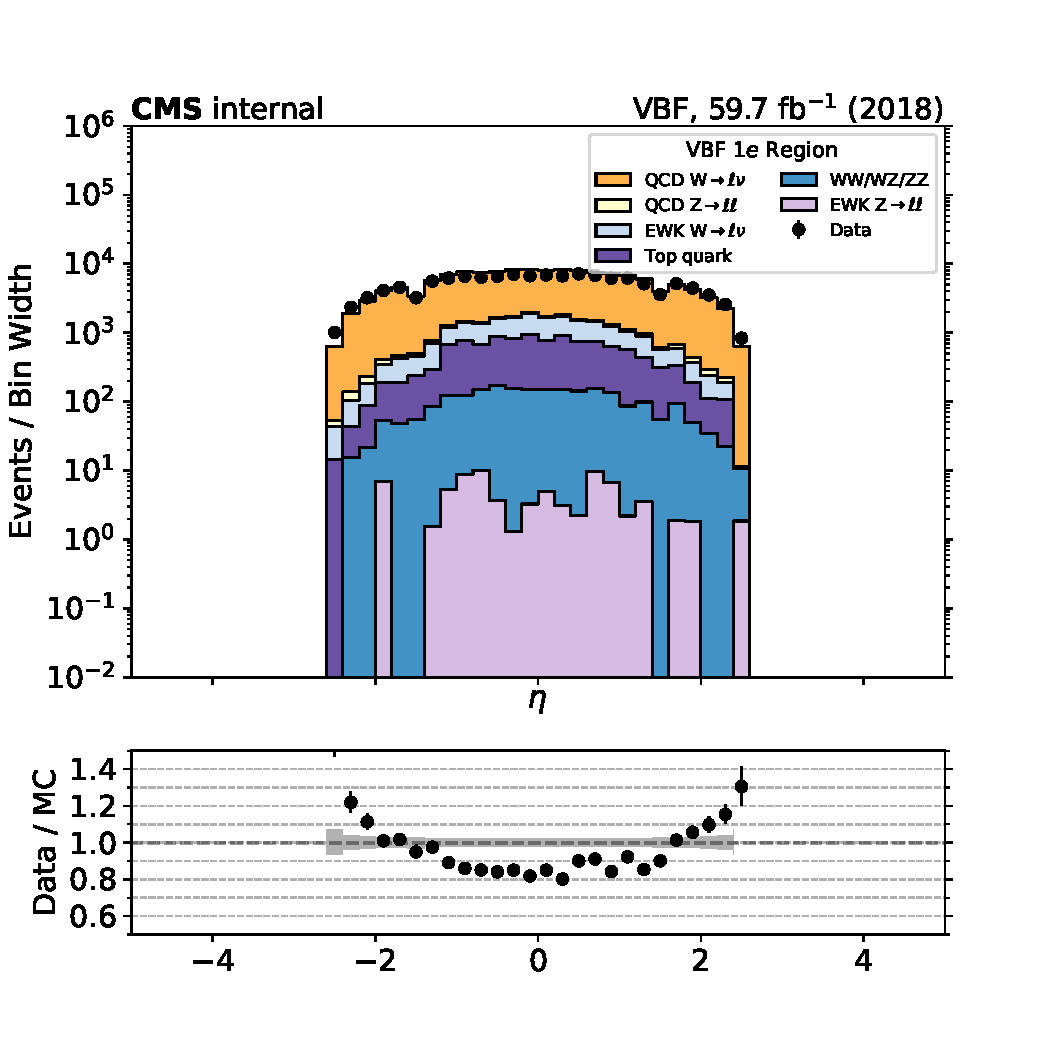
\includegraphics[width=0.49\textwidth]{\plotDir/cr_1e_vbf/cr_1e_vbf_data_mc_electron_eta_2018.pdf}
    \end{center}
    \caption{Comparison between 2018 data and Monte Carlo simulation in the single electron control region. Top plots
    show the $\mjj$ and $\detajj$ distributions for the two leading AK4 jets. Bottom plots show the $\pt$ and $\eta$
    of the reconstructed electron.}
    \label{fig:cr_1e_vbf_2018_mtr}
\end{figure}

\clearpage

\subsection{Double Muon Control Region}
\label{sec:selection_cr_2m}

Double-muon control region events are selected using full signal-region criteria of VBF category with the exception of the muon veto. 
In the double-muon control region, events are selected by requiring leading (subleading) muon \pt greater than 20 (10) GeV and 
an invariant mass of the two muons is required to be in the range of 60 to 120 GeV, compatible with a $\textrm{Z} \rightarrow \mu \mu$ decay. 
At least one of the two muons is required to 
pass the tight candidate definition, as defined in Sec.~\ref{subsec:muons}. 
Events are rejected if there is an additional loose muon or electron with $\pt > 10$ GeV. 
The SR \ptmiss requirement is replaced with an identical requirement on the hadronic recoil, 
which is defined as the sum of \ptvecmiss 
and the muon \vpt (Eq.~\ref{eq:recoil_def}), and thus corresponds to the distribution of the Z \pt smeared
with the $\ptmiss$ resolution of the detector.

Figs.~\ref{fig:cr_2m_vbf_2017_mtr} and~\ref{fig:cr_2m_vbf_2018_mtr} show the distributions of the recoil, $\mjj$, $\detajj$ and  
$\dphijj$ of the two leading AK4 jets for events in the double-muon control region for the VBF category 
in 2017 and 2018 datasets, respectively. Figs.~\ref{fig:cr_2m_vbf_2017_mtr_2} and~\ref{fig:cr_2m_vbf_2018_mtr_2} show the distributions 
of the leading muon \pt and $\eta$, as well as the dimuon mass and minimum $\dphi$ between 4 leading jets and recoil, for 2017 and 2018, respectively.

\begin{figure}[htbp]
    \begin{center}
        \includegraphics[width=0.49\textwidth]{\plotDir/cr_2m_vbf/cr_2m_vbf_data_mc_recoil_2017.pdf}
        \includegraphics[width=0.49\textwidth]{\plotDir/cr_2m_vbf/cr_2m_vbf_data_mc_mjj_2017.pdf} \\
        \includegraphics[width=0.49\textwidth]{\plotDir/cr_2m_vbf/cr_2m_vbf_data_mc_detajj_2017.pdf}
        \includegraphics[width=0.49\textwidth]{\plotDir/cr_2m_vbf/cr_2m_vbf_data_mc_dphijj_2017.pdf}
    \end{center}
    \caption{Comparison between 2017 data and Monte Carlo simulation in the double muon control region for
        the recoil, $\mjj$ distribution, $\detajj$ and $\dphijj$ distributions for the two leading AK4 jets.}
    \label{fig:cr_2m_vbf_2017_mtr}
\end{figure}

\begin{figure}[htbp]
    \begin{center}
        \includegraphics[width=0.49\textwidth]{\plotDir/cr_2m_vbf/cr_2m_vbf_data_mc_muon_pt0_2017.pdf}
        \includegraphics[width=0.49\textwidth]{\plotDir/cr_2m_vbf/cr_2m_vbf_data_mc_muon_eta0_2017.pdf}
        \includegraphics[width=0.49\textwidth]{\plotDir/cr_2m_vbf/cr_2m_vbf_data_mc_dimuon_mass_2017.pdf}
        \includegraphics[width=0.49\textwidth]{\plotDir/cr_2m_vbf/cr_2m_vbf_data_mc_dphijr_2017.pdf}
    \end{center}
    \caption{Comparison between 2017 data and Monte Carlo simulation in the double muon control region for
        the $\pt$ and $\eta$ of the leading muon (top), and dimuon mass and minimum $\dphi$ between 4 leading jets and recoil (bottom).}
    \label{fig:cr_2m_vbf_2017_mtr_2}
\end{figure}

\begin{figure}[htbp]
    \begin{center}
        \includegraphics[width=0.49\textwidth]{\plotDir/cr_2m_vbf/cr_2m_vbf_data_mc_recoil_2018.pdf}
        \includegraphics[width=0.49\textwidth]{\plotDir/cr_2m_vbf/cr_2m_vbf_data_mc_mjj_2018.pdf} \\
        \includegraphics[width=0.49\textwidth]{\plotDir/cr_2m_vbf/cr_2m_vbf_data_mc_detajj_2018.pdf}
        \includegraphics[width=0.49\textwidth]{\plotDir/cr_2m_vbf/cr_2m_vbf_data_mc_dphijj_2018.pdf}
    \end{center}
    \caption{Comparison between 2018 data and Monte Carlo simulation in the double muon control region for
        the recoil, $\mjj$ distribution, $\detajj$ and $\dphijj$ distributions for the two leading AK4 jets.}
    \label{fig:cr_2m_vbf_2018_mtr}
\end{figure}

\begin{figure}[htbp]
    \begin{center}
        \includegraphics[width=0.49\textwidth]{\plotDir/cr_2m_vbf/cr_2m_vbf_data_mc_muon_pt0_2018.pdf}
        \includegraphics[width=0.49\textwidth]{\plotDir/cr_2m_vbf/cr_2m_vbf_data_mc_muon_eta0_2018.pdf}
        \includegraphics[width=0.49\textwidth]{\plotDir/cr_2m_vbf/cr_2m_vbf_data_mc_dimuon_mass_2018.pdf}
        \includegraphics[width=0.49\textwidth]{\plotDir/cr_2m_vbf/cr_2m_vbf_data_mc_dphijr_2018.pdf}
    \end{center}
    \caption{Comparison between 2018 data and Monte Carlo simulation in the double muon control region for
        the $\pt$ and $\eta$ of the leading muon (top), dimuon mass and minimum $\dphi$ between 4 leading jets and recoil (bottom).}
    \label{fig:cr_2m_vbf_2018_mtr_2}
\end{figure}

\clearpage

\subsection{Double Electron Control Region}
\label{sec:selection_cr_2e}

Events for the double-electron control region are collected with the single-electron and 
photon triggers described in Sec.~\ref{subsec:trigger_eff_reweighting}. In the offline analysis, events in the dielectron 
control region are required to contain exactly two oppositely charged electrons with leading (trailing) 
electron \pt greater than 40 (10) GeV, with at least one of the two passing the tight candidate definition, as defined in Sec.~\ref{subsec:electrons}.
Similar to the double-muon region, the invariant mass of the electron-positron pair is required to be in the range of $60$ to $120$ GeV,
thus being compatible with a $\textrm{Z} \rightarrow ee$ decay. 
The SR \ptmiss requirement is replaced with an identical requirement on the hadronic recoil, which is defined as the 
sum of \ptvecmiss and the electron \vpt (Eq.~\ref{eq:recoil_def}), and thus corresponds to the distribution of the Z \pt smeared with the \ptmiss resolution. 

Figs.~\ref{fig:cr_2e_vbf_2017_mtr} and~\ref{fig:cr_2e_vbf_2018_mtr} show the distributions of the recoil, $\mjj$, $\detajj$ and
$\dphijj$ for the two leading AK4 jets for events in the double-electron control region for the VBF category 
in 2017 and 2018 datasets, respectively. 
Figs.~\ref{fig:cr_2e_vbf_2017_mtr_2} and~\ref{fig:cr_2e_vbf_2018_mtr_2} show the distributions of the leading electron \pt and $\eta$, 
as well as the dielectron mass and minimum $\dphi$ between 4 leading jets and recoil, for 2017 and 2018, respectively.

\begin{figure}[htbp]
    \begin{center}
        \includegraphics[width=0.49\textwidth]{\plotDir/cr_2e_vbf/cr_2e_vbf_data_mc_recoil_2017.pdf}
        \includegraphics[width=0.49\textwidth]{\plotDir/cr_2e_vbf/cr_2e_vbf_data_mc_mjj_2017.pdf} \\
        \includegraphics[width=0.49\textwidth]{\plotDir/cr_2e_vbf/cr_2e_vbf_data_mc_detajj_2017.pdf}
        \includegraphics[width=0.49\textwidth]{\plotDir/cr_2e_vbf/cr_2e_vbf_data_mc_dphijj_2017.pdf}
    \end{center}
    \caption{Comparison between 2017 data and Monte Carlo simulation in the double electron control region for
        the recoil, $\mjj$ distribution, $\detajj$ and $\dphijj$ distributions for the two leading AK4 jets.}
    \label{fig:cr_2e_vbf_2017_mtr}
\end{figure}

\begin{figure}[htbp]
    \begin{center}
        \includegraphics[width=0.49\textwidth]{\plotDir/cr_2e_vbf/cr_2e_vbf_data_mc_electron_pt0_2017.pdf}
        \includegraphics[width=0.49\textwidth]{\plotDir/cr_2e_vbf/cr_2e_vbf_data_mc_electron_eta0_2017.pdf}
        \includegraphics[width=0.49\textwidth]{\plotDir/cr_2e_vbf/cr_2e_vbf_data_mc_dielectron_mass_2017.pdf}
        \includegraphics[width=0.49\textwidth]{\plotDir/cr_2e_vbf/cr_2e_vbf_data_mc_dphijr_2017.pdf}
    \end{center}
    \caption{Comparison between 2017 data and Monte Carlo simulation in the double electron control region for
        the $\pt$ and $\eta$ of the leading electron (top), dielectron mass and minimum $\dphi$ between 4 leading jets and recoil (bottom).}
    \label{fig:cr_2e_vbf_2017_mtr_2}
\end{figure}

\begin{figure}[htbp]
    \begin{center}
        \includegraphics[width=0.49\textwidth]{\plotDir/cr_2e_vbf/cr_2e_vbf_data_mc_recoil_2018.pdf}
        \includegraphics[width=0.49\textwidth]{\plotDir/cr_2e_vbf/cr_2e_vbf_data_mc_mjj_2018.pdf} \\
        \includegraphics[width=0.49\textwidth]{\plotDir/cr_2e_vbf/cr_2e_vbf_data_mc_detajj_2018.pdf}
        \includegraphics[width=0.49\textwidth]{\plotDir/cr_2e_vbf/cr_2e_vbf_data_mc_dphijj_2018.pdf}
    \end{center}
    \caption{Comparison between 2018 data and Monte Carlo simulation in the double electron control region for
        the recoil, $\mjj$ distribution, $\detajj$ and $\dphijj$ distributions for the two leading AK4 jets.}
    \label{fig:cr_2e_vbf_2018_mtr}
\end{figure}

\begin{figure}[htbp]
    \begin{center}
        \includegraphics[width=0.49\textwidth]{\plotDir/cr_2e_vbf/cr_2e_vbf_data_mc_electron_pt0_2018.pdf}
        \includegraphics[width=0.49\textwidth]{\plotDir/cr_2e_vbf/cr_2e_vbf_data_mc_electron_eta0_2018.pdf}
        \includegraphics[width=0.49\textwidth]{\plotDir/cr_2e_vbf/cr_2e_vbf_data_mc_dielectron_mass_2018.pdf}
        \includegraphics[width=0.49\textwidth]{\plotDir/cr_2e_vbf/cr_2e_vbf_data_mc_dphijr_2018.pdf}
    \end{center}
    \caption{Comparison between 2018 data and Monte Carlo simulation in the double electron control region for
        the $\pt$ and $\eta$ of the leading electron (top), dielectron mass and minimum $\dphi$ between 4 leading jets and recoil (bottom).}
    \label{fig:cr_2e_vbf_2018_mtr_2}
\end{figure}

\clearpage

\subsection{Photon Control Region}
\label{sec:selection_cr_g}

To further constrain the \Zvv \ background in the signal region, a photon control region is used.
At large transverse momenta, the kinematic properties of photon production become similar to those of the $\Zvv$ process, 
and can therefore be used to estimate the latter. Events for the control region are selected using a trigger requiring 
an online photon \pt of at least $200$ GeV. In the offline analysis, photons are required to be located in the barrel 
part of the detector ($|\eta|<1.4442$), have transverse momenta of at least $230$ GeV to ensure full trigger efficiency, 
and pass additional identification criteria based on the properties of the associated supercluster in the ECAL, 
as well as the isolation of the photon relative to nearby energy objects. To be considered for the control region, 
events must have exactly one such photon, with no additional photons or leptons passing the loose criteria described above. 
Jets and hadronic recoil are required to pass criteria identical to those imposed in the signal region, where the recoil 
is defined as as the vectorial sum of \ptvecmiss and the photon transverse momentum (Eq.~\ref{eq:recoil_def}).

Figs.~\ref{fig:Photon_vbfhinv_2017} and~\ref{fig:Photon_vbfhinv_2018} show the distributions of the recoil, $\mjj$, $\detajj$ and 
$\dphijj$ distributions of the two leading AK4 jets for events in the photon control region for the VBF category in the 
2017 and 2018 datasets, respectively. Similarly, Figs.~\ref{fig:Photon2_vbfhinv_2017} and~\ref{fig:Photon2_vbfhinv_2018} 
show the distributions of the photon $\pt$ and $\eta$.

\begin{figure}[htbp]
    \begin{center}
        \includegraphics[width=0.49\textwidth]{\plotDir/cr_g_vbf/cr_g_vbf_data_mc_recoil_2017.pdf}
        \includegraphics[width=0.49\textwidth]{\plotDir/cr_g_vbf/cr_g_vbf_data_mc_mjj_2017.pdf} \\
        \includegraphics[width=0.49\textwidth]{\plotDir/cr_g_vbf/cr_g_vbf_data_mc_detajj_2017.pdf}
        \includegraphics[width=0.49\textwidth]{\plotDir/cr_g_vbf/cr_g_vbf_data_mc_dphijj_2017.pdf}
    \end{center}
    \caption{Comparison between 2017 data and Monte Carlo simulation in the photon control region for
        the recoil distribution, the $\mjj$ distribution, $\detajj$ distribution and $\dphijj$ distribution
        for the two leading AK4 jets. The $\mjj$ and recoil distributions include the QCD estimate
        calculated from the photon purity measurement, as described in Sec.~\ref{subsec:photonpurity}. }
    \label{fig:Photon_vbfhinv_2017}
\end{figure}

\begin{figure}[htbp]
    \begin{center}
        \includegraphics[width=0.49\textwidth]{\plotDir/cr_g_vbf/cr_g_vbf_data_mc_photon_pt0_2017.pdf}
        \includegraphics[width=0.49\textwidth]{\plotDir/cr_g_vbf/cr_g_vbf_data_mc_photon_eta0_2017.pdf}
    \end{center}
    \caption{Comparison between 2017 data and Monte Carlo simulation in the photon control region for
        the $\pt$ and $\eta$ of the leading photon.}
    \label{fig:Photon2_vbfhinv_2017}
\end{figure}

\begin{figure}[htbp]
    \begin{center}
        \includegraphics[width=0.49\textwidth]{\plotDir/cr_g_vbf/cr_g_vbf_data_mc_recoil_2018.pdf}
        \includegraphics[width=0.49\textwidth]{\plotDir/cr_g_vbf/cr_g_vbf_data_mc_mjj_2018.pdf} \\
        \includegraphics[width=0.49\textwidth]{\plotDir/cr_g_vbf/cr_g_vbf_data_mc_detajj_2018.pdf}
        \includegraphics[width=0.49\textwidth]{\plotDir/cr_g_vbf/cr_g_vbf_data_mc_dphijj_2018.pdf}
    \end{center}
    \caption{Comparison between 2018 data and Monte Carlo simulation in the photon control region for
        the recoil distribution, the $\mjj$ distribution, $\detajj$ distribution and $\dphijj$ distribution
        for the two leading AK4 jets. The $\mjj$ and recoil distributions include the QCD estimate
        calculated from the photon purtiy measurement, as described in Sec.~\ref{subsec:photonpurity}. }
    \label{fig:Photon_vbfhinv_2018}
\end{figure}

\begin{figure}[htbp]
    \begin{center}
        \includegraphics[width=0.49\textwidth]{\plotDir/cr_g_vbf/cr_g_vbf_data_mc_photon_pt0_2018.pdf}
        \includegraphics[width=0.49\textwidth]{\plotDir/cr_g_vbf/cr_g_vbf_data_mc_photon_eta0_2018.pdf}
    \end{center}
    \caption{Comparison between 2018 data and Monte Carlo simulation in the photon control region for
        the $\pt$ and $\eta$ of the leading photon.}
    \label{fig:Photon2_vbfhinv_2018}
\end{figure}

\clearpage